% Generated by Sphinx.
\def\sphinxdocclass{report}
\documentclass[letterpaper,10pt,english]{sphinxmanual}
\usepackage[utf8]{inputenc}
\DeclareUnicodeCharacter{00A0}{\nobreakspace}
\usepackage{cmap}
\usepackage[T1]{fontenc}
\usepackage{babel}
\usepackage{times}
\usepackage[Bjarne]{fncychap}
\usepackage{longtable}
\usepackage{sphinx}
\usepackage{multirow}

\addto\captionsenglish{\renewcommand{\figurename}{Fig. }}
\addto\captionsenglish{\renewcommand{\tablename}{Table }}
\floatname{literal-block}{Listing }



\title{saegus Documentation}
\date{April 04, 2016}
\release{0.1.2}
\author{John J. Dougherty III}
\newcommand{\sphinxlogo}{}
\renewcommand{\releasename}{Release}
\makeindex

\makeatletter
\def\PYG@reset{\let\PYG@it=\relax \let\PYG@bf=\relax%
    \let\PYG@ul=\relax \let\PYG@tc=\relax%
    \let\PYG@bc=\relax \let\PYG@ff=\relax}
\def\PYG@tok#1{\csname PYG@tok@#1\endcsname}
\def\PYG@toks#1+{\ifx\relax#1\empty\else%
    \PYG@tok{#1}\expandafter\PYG@toks\fi}
\def\PYG@do#1{\PYG@bc{\PYG@tc{\PYG@ul{%
    \PYG@it{\PYG@bf{\PYG@ff{#1}}}}}}}
\def\PYG#1#2{\PYG@reset\PYG@toks#1+\relax+\PYG@do{#2}}

\expandafter\def\csname PYG@tok@nc\endcsname{\let\PYG@bf=\textbf\def\PYG@tc##1{\textcolor[rgb]{0.05,0.52,0.71}{##1}}}
\expandafter\def\csname PYG@tok@c1\endcsname{\let\PYG@it=\textit\def\PYG@tc##1{\textcolor[rgb]{0.25,0.50,0.56}{##1}}}
\expandafter\def\csname PYG@tok@ch\endcsname{\let\PYG@it=\textit\def\PYG@tc##1{\textcolor[rgb]{0.25,0.50,0.56}{##1}}}
\expandafter\def\csname PYG@tok@ow\endcsname{\let\PYG@bf=\textbf\def\PYG@tc##1{\textcolor[rgb]{0.00,0.44,0.13}{##1}}}
\expandafter\def\csname PYG@tok@s1\endcsname{\def\PYG@tc##1{\textcolor[rgb]{0.25,0.44,0.63}{##1}}}
\expandafter\def\csname PYG@tok@gs\endcsname{\let\PYG@bf=\textbf}
\expandafter\def\csname PYG@tok@si\endcsname{\let\PYG@it=\textit\def\PYG@tc##1{\textcolor[rgb]{0.44,0.63,0.82}{##1}}}
\expandafter\def\csname PYG@tok@kd\endcsname{\let\PYG@bf=\textbf\def\PYG@tc##1{\textcolor[rgb]{0.00,0.44,0.13}{##1}}}
\expandafter\def\csname PYG@tok@w\endcsname{\def\PYG@tc##1{\textcolor[rgb]{0.73,0.73,0.73}{##1}}}
\expandafter\def\csname PYG@tok@s2\endcsname{\def\PYG@tc##1{\textcolor[rgb]{0.25,0.44,0.63}{##1}}}
\expandafter\def\csname PYG@tok@nd\endcsname{\let\PYG@bf=\textbf\def\PYG@tc##1{\textcolor[rgb]{0.33,0.33,0.33}{##1}}}
\expandafter\def\csname PYG@tok@cs\endcsname{\def\PYG@tc##1{\textcolor[rgb]{0.25,0.50,0.56}{##1}}\def\PYG@bc##1{\setlength{\fboxsep}{0pt}\colorbox[rgb]{1.00,0.94,0.94}{\strut ##1}}}
\expandafter\def\csname PYG@tok@mb\endcsname{\def\PYG@tc##1{\textcolor[rgb]{0.13,0.50,0.31}{##1}}}
\expandafter\def\csname PYG@tok@sc\endcsname{\def\PYG@tc##1{\textcolor[rgb]{0.25,0.44,0.63}{##1}}}
\expandafter\def\csname PYG@tok@gp\endcsname{\let\PYG@bf=\textbf\def\PYG@tc##1{\textcolor[rgb]{0.78,0.36,0.04}{##1}}}
\expandafter\def\csname PYG@tok@mi\endcsname{\def\PYG@tc##1{\textcolor[rgb]{0.13,0.50,0.31}{##1}}}
\expandafter\def\csname PYG@tok@vg\endcsname{\def\PYG@tc##1{\textcolor[rgb]{0.73,0.38,0.84}{##1}}}
\expandafter\def\csname PYG@tok@bp\endcsname{\def\PYG@tc##1{\textcolor[rgb]{0.00,0.44,0.13}{##1}}}
\expandafter\def\csname PYG@tok@il\endcsname{\def\PYG@tc##1{\textcolor[rgb]{0.13,0.50,0.31}{##1}}}
\expandafter\def\csname PYG@tok@gi\endcsname{\def\PYG@tc##1{\textcolor[rgb]{0.00,0.63,0.00}{##1}}}
\expandafter\def\csname PYG@tok@nf\endcsname{\def\PYG@tc##1{\textcolor[rgb]{0.02,0.16,0.49}{##1}}}
\expandafter\def\csname PYG@tok@kn\endcsname{\let\PYG@bf=\textbf\def\PYG@tc##1{\textcolor[rgb]{0.00,0.44,0.13}{##1}}}
\expandafter\def\csname PYG@tok@ge\endcsname{\let\PYG@it=\textit}
\expandafter\def\csname PYG@tok@sx\endcsname{\def\PYG@tc##1{\textcolor[rgb]{0.78,0.36,0.04}{##1}}}
\expandafter\def\csname PYG@tok@na\endcsname{\def\PYG@tc##1{\textcolor[rgb]{0.25,0.44,0.63}{##1}}}
\expandafter\def\csname PYG@tok@sd\endcsname{\let\PYG@it=\textit\def\PYG@tc##1{\textcolor[rgb]{0.25,0.44,0.63}{##1}}}
\expandafter\def\csname PYG@tok@vi\endcsname{\def\PYG@tc##1{\textcolor[rgb]{0.73,0.38,0.84}{##1}}}
\expandafter\def\csname PYG@tok@ni\endcsname{\let\PYG@bf=\textbf\def\PYG@tc##1{\textcolor[rgb]{0.84,0.33,0.22}{##1}}}
\expandafter\def\csname PYG@tok@mo\endcsname{\def\PYG@tc##1{\textcolor[rgb]{0.13,0.50,0.31}{##1}}}
\expandafter\def\csname PYG@tok@err\endcsname{\def\PYG@bc##1{\setlength{\fboxsep}{0pt}\fcolorbox[rgb]{1.00,0.00,0.00}{1,1,1}{\strut ##1}}}
\expandafter\def\csname PYG@tok@gd\endcsname{\def\PYG@tc##1{\textcolor[rgb]{0.63,0.00,0.00}{##1}}}
\expandafter\def\csname PYG@tok@nn\endcsname{\let\PYG@bf=\textbf\def\PYG@tc##1{\textcolor[rgb]{0.05,0.52,0.71}{##1}}}
\expandafter\def\csname PYG@tok@cpf\endcsname{\let\PYG@it=\textit\def\PYG@tc##1{\textcolor[rgb]{0.25,0.50,0.56}{##1}}}
\expandafter\def\csname PYG@tok@nb\endcsname{\def\PYG@tc##1{\textcolor[rgb]{0.00,0.44,0.13}{##1}}}
\expandafter\def\csname PYG@tok@gt\endcsname{\def\PYG@tc##1{\textcolor[rgb]{0.00,0.27,0.87}{##1}}}
\expandafter\def\csname PYG@tok@kp\endcsname{\def\PYG@tc##1{\textcolor[rgb]{0.00,0.44,0.13}{##1}}}
\expandafter\def\csname PYG@tok@s\endcsname{\def\PYG@tc##1{\textcolor[rgb]{0.25,0.44,0.63}{##1}}}
\expandafter\def\csname PYG@tok@kc\endcsname{\let\PYG@bf=\textbf\def\PYG@tc##1{\textcolor[rgb]{0.00,0.44,0.13}{##1}}}
\expandafter\def\csname PYG@tok@o\endcsname{\def\PYG@tc##1{\textcolor[rgb]{0.40,0.40,0.40}{##1}}}
\expandafter\def\csname PYG@tok@go\endcsname{\def\PYG@tc##1{\textcolor[rgb]{0.20,0.20,0.20}{##1}}}
\expandafter\def\csname PYG@tok@gu\endcsname{\let\PYG@bf=\textbf\def\PYG@tc##1{\textcolor[rgb]{0.50,0.00,0.50}{##1}}}
\expandafter\def\csname PYG@tok@gh\endcsname{\let\PYG@bf=\textbf\def\PYG@tc##1{\textcolor[rgb]{0.00,0.00,0.50}{##1}}}
\expandafter\def\csname PYG@tok@nv\endcsname{\def\PYG@tc##1{\textcolor[rgb]{0.73,0.38,0.84}{##1}}}
\expandafter\def\csname PYG@tok@k\endcsname{\let\PYG@bf=\textbf\def\PYG@tc##1{\textcolor[rgb]{0.00,0.44,0.13}{##1}}}
\expandafter\def\csname PYG@tok@cm\endcsname{\let\PYG@it=\textit\def\PYG@tc##1{\textcolor[rgb]{0.25,0.50,0.56}{##1}}}
\expandafter\def\csname PYG@tok@c\endcsname{\let\PYG@it=\textit\def\PYG@tc##1{\textcolor[rgb]{0.25,0.50,0.56}{##1}}}
\expandafter\def\csname PYG@tok@sr\endcsname{\def\PYG@tc##1{\textcolor[rgb]{0.14,0.33,0.53}{##1}}}
\expandafter\def\csname PYG@tok@m\endcsname{\def\PYG@tc##1{\textcolor[rgb]{0.13,0.50,0.31}{##1}}}
\expandafter\def\csname PYG@tok@cp\endcsname{\def\PYG@tc##1{\textcolor[rgb]{0.00,0.44,0.13}{##1}}}
\expandafter\def\csname PYG@tok@sb\endcsname{\def\PYG@tc##1{\textcolor[rgb]{0.25,0.44,0.63}{##1}}}
\expandafter\def\csname PYG@tok@no\endcsname{\def\PYG@tc##1{\textcolor[rgb]{0.38,0.68,0.84}{##1}}}
\expandafter\def\csname PYG@tok@kt\endcsname{\def\PYG@tc##1{\textcolor[rgb]{0.56,0.13,0.00}{##1}}}
\expandafter\def\csname PYG@tok@vc\endcsname{\def\PYG@tc##1{\textcolor[rgb]{0.73,0.38,0.84}{##1}}}
\expandafter\def\csname PYG@tok@nt\endcsname{\let\PYG@bf=\textbf\def\PYG@tc##1{\textcolor[rgb]{0.02,0.16,0.45}{##1}}}
\expandafter\def\csname PYG@tok@mh\endcsname{\def\PYG@tc##1{\textcolor[rgb]{0.13,0.50,0.31}{##1}}}
\expandafter\def\csname PYG@tok@ne\endcsname{\def\PYG@tc##1{\textcolor[rgb]{0.00,0.44,0.13}{##1}}}
\expandafter\def\csname PYG@tok@sh\endcsname{\def\PYG@tc##1{\textcolor[rgb]{0.25,0.44,0.63}{##1}}}
\expandafter\def\csname PYG@tok@se\endcsname{\let\PYG@bf=\textbf\def\PYG@tc##1{\textcolor[rgb]{0.25,0.44,0.63}{##1}}}
\expandafter\def\csname PYG@tok@mf\endcsname{\def\PYG@tc##1{\textcolor[rgb]{0.13,0.50,0.31}{##1}}}
\expandafter\def\csname PYG@tok@ss\endcsname{\def\PYG@tc##1{\textcolor[rgb]{0.32,0.47,0.09}{##1}}}
\expandafter\def\csname PYG@tok@gr\endcsname{\def\PYG@tc##1{\textcolor[rgb]{1.00,0.00,0.00}{##1}}}
\expandafter\def\csname PYG@tok@nl\endcsname{\let\PYG@bf=\textbf\def\PYG@tc##1{\textcolor[rgb]{0.00,0.13,0.44}{##1}}}
\expandafter\def\csname PYG@tok@kr\endcsname{\let\PYG@bf=\textbf\def\PYG@tc##1{\textcolor[rgb]{0.00,0.44,0.13}{##1}}}

\def\PYGZbs{\char`\\}
\def\PYGZus{\char`\_}
\def\PYGZob{\char`\{}
\def\PYGZcb{\char`\}}
\def\PYGZca{\char`\^}
\def\PYGZam{\char`\&}
\def\PYGZlt{\char`\<}
\def\PYGZgt{\char`\>}
\def\PYGZsh{\char`\#}
\def\PYGZpc{\char`\%}
\def\PYGZdl{\char`\$}
\def\PYGZhy{\char`\-}
\def\PYGZsq{\char`\'}
\def\PYGZdq{\char`\"}
\def\PYGZti{\char`\~}
% for compatibility with earlier versions
\def\PYGZat{@}
\def\PYGZlb{[}
\def\PYGZrb{]}
\makeatother

\renewcommand\PYGZsq{\textquotesingle}

\begin{document}

\maketitle
\tableofcontents
\phantomsection\label{contents::doc}


Contents:


\chapter{MAGIC Population with Subset of Loci}
\label{magic1478:magic-population-with-subset-of-loci}\label{magic1478:welcome-to-saegus-s-documentation}\label{magic1478::doc}
The \code{standard\_magic} population uses all 7386 loci from \code{hapmap3.txt}. However,
if I use all 7386 loci and the triplet scheme this alters the GWAS results. I need
to create a population which uses the loci which occupy integer-valued positions on the
genetic map i.e. 1.0 cM, 2.0 cM. \code{standard\_magic} has the loci at 0.6 cM, 0.8 cM, 1.0 cM, 1.2 cM
so on and so forth.


\section{Allele Effects and Triplets of Non-Recombining Loci}
\label{magic1478:allele-effects-and-triplets-of-non-recombining-loci}
The \code{standard\_magic} population assigns effects to an integer-valued position
and the positions immediately upstream and downstream. When I use the subset of 1478 loci
I will assign the alleles at those loci effects as \textbf{three independent} draws from
an exponential distribution. The goal is to make \code{magic1478} somewhat comparable to \code{standard\_magic}.


\section{Strategy of Creating MAGIC1478}
\label{magic1478:strategy-of-creating-magic1478}
I am going to use the \code{nam\_prefounders} and withdraw the integer-valued positions of each individual.
This saves me the work of building up the population from the raw files.


\subsection{Creating the simuPOP Population Object for MAGIC1478}
\label{magic1478:creating-the-simupop-population-object-for-magic1478}
A simuPOP \code{Population} requires the number of chromosomes and the number of loci per chromosome.
Luckily I saved the absolute indexes of the integer-valued positions of the genetic map in a
\code{shelve} instance.

\begin{Verbatim}[commandchars=\\\{\}]
\PYG{n}{misc\PYGZus{}gmap} \PYG{o}{=} \PYG{n}{shelve}\PYG{o}{.}\PYG{n}{open}\PYG{p}{(}\PYG{l+s+s1}{\PYGZsq{}}\PYG{l+s+s1}{misc\PYGZus{}gmap}\PYG{l+s+s1}{\PYGZsq{}}\PYG{p}{)}
\PYG{n}{integral\PYGZus{}valued\PYGZus{}loci} \PYG{o}{=} \PYG{n}{misc\PYGZus{}gmap}\PYG{p}{[}\PYG{l+s+s1}{\PYGZsq{}}\PYG{l+s+s1}{integral\PYGZus{}valued\PYGZus{}loci}\PYG{l+s+s1}{\PYGZsq{}}\PYG{p}{]}
\PYG{n}{relative\PYGZus{}integral\PYGZus{}valued\PYGZus{}loci} \PYG{o}{=} \PYG{n}{misc\PYGZus{}gmap}\PYG{p}{[}\PYG{l+s+s1}{\PYGZsq{}}\PYG{l+s+s1}{relative\PYGZus{}integral\PYGZus{}valued\PYGZus{}loci}\PYG{l+s+s1}{\PYGZsq{}}\PYG{p}{]}
\PYG{k}{print}\PYG{p}{(}\PYG{n}{integral\PYGZus{}valued\PYGZus{}loci}\PYG{p}{[}\PYG{p}{:}\PYG{l+m+mi}{10}\PYG{p}{]}\PYG{p}{)}
\PYG{p}{[}\PYG{l+m+mi}{4}\PYG{p}{,} \PYG{l+m+mi}{9}\PYG{p}{,} \PYG{l+m+mi}{14}\PYG{p}{,} \PYG{l+m+mi}{19}\PYG{p}{,} \PYG{l+m+mi}{24}\PYG{p}{,} \PYG{l+m+mi}{29}\PYG{p}{,} \PYG{l+m+mi}{34}\PYG{p}{,} \PYG{l+m+mi}{39}\PYG{p}{,} \PYG{l+m+mi}{44}\PYG{p}{,} \PYG{l+m+mi}{49}\PYG{p}{]}
\end{Verbatim}

\code{relative\_integral\_valued\_loci} is a \code{dict} which is keyed by absolute locus index. We will extract the chromosome
of each absolute valued index and then use \code{collections.Counter} to count how many loci are on each chromosome.

\begin{Verbatim}[commandchars=\\\{\}]
\PYG{k}{print}\PYG{p}{(}\PYG{n}{relative\PYGZus{}integral\PYGZus{}valued\PYGZus{}loci}\PYG{p}{[}\PYG{l+m+mi}{4}\PYG{p}{]}\PYG{p}{)}
\PYG{p}{(}\PYG{l+m+mi}{1}\PYG{p}{,} \PYG{o}{\PYGZhy{}}\PYG{l+m+mf}{4.0}\PYG{p}{)}

\PYG{n}{integer\PYGZus{}loci\PYGZus{}per\PYGZus{}chromosome} \PYG{o}{=} \PYG{p}{[}\PYG{n}{relative\PYGZus{}integral\PYGZus{}valued\PYGZus{}loci}\PYG{p}{[}\PYG{n}{abs\PYGZus{}locus}\PYG{p}{]}\PYG{p}{[}\PYG{l+m+mi}{0}\PYG{p}{]} \PYG{k}{for} \PYG{n}{abs\PYGZus{}locus} \PYG{o+ow}{in} \PYG{n}{integral\PYGZus{}valued\PYGZus{}loci}\PYG{p}{]}

\PYG{k+kn}{import} \PYG{n+nn}{collections} \PYG{k+kn}{as} \PYG{n+nn}{col}

\PYG{n}{integer\PYGZus{}valued\PYGZus{}loci\PYGZus{}per\PYGZus{}chromosome} \PYG{o}{=} \PYG{n}{col}\PYG{o}{.}\PYG{n}{Counter}\PYG{p}{(}\PYG{n}{loci\PYGZus{}per\PYGZus{}chromosome}\PYG{p}{)}
\PYG{k}{print}\PYG{p}{(}\PYG{n}{integer\PYGZus{}valued\PYGZus{}loci\PYGZus{}per\PYGZus{}chromosome}\PYG{p}{)}

\PYG{n}{Counter}\PYG{p}{(}\PYG{p}{\PYGZob{}}\PYG{l+m+mf}{1.0}\PYG{p}{:} \PYG{l+m+mi}{210}\PYG{p}{,} \PYG{l+m+mf}{3.0}\PYG{p}{:} \PYG{l+m+mi}{164}\PYG{p}{,} \PYG{l+m+mf}{2.0}\PYG{p}{:} \PYG{l+m+mi}{161}\PYG{p}{,} \PYG{l+m+mf}{5.0}\PYG{p}{:} \PYG{l+m+mi}{157}\PYG{p}{,} \PYG{l+m+mf}{4.0}\PYG{p}{:} \PYG{l+m+mi}{152}\PYG{p}{,} \PYG{l+m+mf}{7.0}\PYG{p}{:} \PYG{l+m+mi}{139}\PYG{p}{,} \PYG{l+m+mf}{8.0}\PYG{p}{:} \PYG{l+m+mi}{138}\PYG{p}{,} \PYG{l+m+mf}{9.0}\PYG{p}{:} \PYG{l+m+mi}{132}\PYG{p}{,} \PYG{l+m+mf}{10.0}\PYG{p}{:} \PYG{l+m+mi}{113}\PYG{p}{,} \PYG{l+m+mf}{6.0}\PYG{p}{:} \PYG{l+m+mi}{112}\PYG{p}{\PYGZcb{}}\PYG{p}{)}

\PYG{n}{loci\PYGZus{}per\PYGZus{}chromosome} \PYG{o}{=} \PYG{n+nb}{tuple}\PYG{p}{(}\PYG{n}{integer\PYGZus{}valued\PYGZus{}loci\PYGZus{}per\PYGZus{}chromosome}\PYG{o}{.}\PYG{n}{values}\PYG{p}{(}\PYG{p}{)}\PYG{p}{)}

\PYG{k}{print}\PYG{p}{(}\PYG{n}{loci\PYGZus{}per\PYGZus{}chromosome}\PYG{p}{)}
\PYG{p}{(}\PYG{l+m+mi}{210}\PYG{p}{,} \PYG{l+m+mi}{161}\PYG{p}{,} \PYG{l+m+mi}{164}\PYG{p}{,} \PYG{l+m+mi}{152}\PYG{p}{,} \PYG{l+m+mi}{157}\PYG{p}{,} \PYG{l+m+mi}{112}\PYG{p}{,} \PYG{l+m+mi}{139}\PYG{p}{,} \PYG{l+m+mi}{138}\PYG{p}{,} \PYG{l+m+mi}{132}\PYG{p}{,} \PYG{l+m+mi}{113}\PYG{p}{)}
\end{Verbatim}

So then I can simply do:

\begin{Verbatim}[commandchars=\\\{\}]
\PYG{n}{prefounders\PYGZus{}1478} \PYG{o}{=} \PYG{n}{sim}\PYG{o}{.}\PYG{n}{Population}\PYG{p}{(}\PYG{n}{size}\PYG{o}{=}\PYG{l+m+mi}{26}\PYG{p}{,} \PYG{n}{ploidy}\PYG{o}{=}\PYG{l+m+mi}{2}\PYG{p}{,} \PYG{n}{loci}\PYG{o}{=}\PYG{n}{loci\PYGZus{}per\PYGZus{}chromosome}\PYG{p}{)}
\end{Verbatim}

This initializes the population and now I can copy over genotypes at the integer valued positions from
the prefounders7386 population.

\begin{Verbatim}[commandchars=\\\{\}]
\PYG{n}{prefounders7386} \PYG{o}{=} \PYG{n}{sim}\PYG{o}{.}\PYG{n}{loadPopulation}\PYG{p}{(}\PYG{l+s+s1}{\PYGZsq{}}\PYG{l+s+s1}{nam\PYGZus{}prefounders.pop}\PYG{l+s+s1}{\PYGZsq{}}\PYG{p}{)}
\PYG{k}{for} \PYG{n}{ind\PYGZus{}7386}\PYG{p}{,} \PYG{n}{ind\PYGZus{}1478} \PYG{o+ow}{in} \PYG{n+nb}{zip}\PYG{p}{(}\PYG{n}{prefounders\PYGZus{}7386}\PYG{o}{.}\PYG{n}{individuals}\PYG{p}{(}\PYG{p}{)}\PYG{p}{,} \PYG{n}{prefounders\PYGZus{}1478}\PYG{o}{.}\PYG{n}{individuals}\PYG{p}{(}\PYG{p}{)}\PYG{p}{)}\PYG{p}{:}
   \PYG{n}{sub\PYGZus{}alpha} \PYG{o}{=} \PYG{p}{[}\PYG{n}{ind\PYGZus{}7386}\PYG{o}{.}\PYG{n}{genotype}\PYG{p}{(}\PYG{n}{ploidy}\PYG{o}{=}\PYG{l+m+mi}{0}\PYG{p}{)}\PYG{p}{[}\PYG{n}{integer\PYGZus{}position}\PYG{p}{]}
               \PYG{k}{for} \PYG{n}{integer\PYGZus{}position} \PYG{o+ow}{in} \PYG{n}{integer\PYGZus{}subset}\PYG{p}{]}
   \PYG{n}{sub\PYGZus{}beta} \PYG{o}{=} \PYG{p}{[}\PYG{n}{ind\PYGZus{}7386}\PYG{o}{.}\PYG{n}{genotype}\PYG{p}{(}\PYG{n}{ploidy}\PYG{o}{=}\PYG{l+m+mi}{1}\PYG{p}{)}\PYG{p}{[}\PYG{n}{integer\PYGZus{}position}\PYG{p}{]}
              \PYG{k}{for} \PYG{n}{integer\PYGZus{}position} \PYG{o+ow}{in} \PYG{n}{integer\PYGZus{}subset}\PYG{p}{]}
   \PYG{n}{genotype\PYGZus{}1478} \PYG{o}{=} \PYG{n}{sub\PYGZus{}alpha} \PYG{o}{+} \PYG{n}{sub\PYGZus{}beta}
   \PYG{n}{ind\PYGZus{}1478}\PYG{o}{.}\PYG{n}{setGenotype}\PYG{p}{(}\PYG{n}{genotype\PYGZus{}1478}\PYG{p}{)}
\end{Verbatim}


\section{Generating Standard MAGIC1478 from Prefounders1478}
\label{magic1478:making-prefounders-1478}\label{magic1478:generating-standard-magic1478-from-prefounders1478}
I followed the same mating and testing strategy to make a \code{standard\_magic\_1478.pop} file. I used
the same founders as in \code{standard\_magic} i.e. founders 1 through 8.

\begin{Verbatim}[commandchars=\\\{\}]
\PYG{n}{prefounders\PYGZus{}1478} \PYG{o}{=} \PYG{n}{sim}\PYG{o}{.}\PYG{n}{loadPopulation}\PYG{p}{(}\PYG{l+s+s1}{\PYGZsq{}}\PYG{l+s+s1}{prefounders\PYGZus{}1478.pop}\PYG{l+s+s1}{\PYGZsq{}}\PYG{p}{)}
\end{Verbatim}


\subsection{Determine the Mating Pairs of Each Generation}
\label{magic1478:determine-the-mating-pairs-of-each-generation}
I created a standardized MAGIC1478 population as I did with MAGIC7386. At each step
I pre-determine the mating pairs and record them in \code{lists} which have the title
\code{expected\_x\_mother\_ids} and \code{expected\_x\_father\_ids}. The expected parental id pairs are
mated in order. The offspring have infoFields which record the ID of their mother and ID father.

After mating the offspring parental IDs are compared with the expected parental IDs.
Below is an example of this mating-testing cycle.

\begin{Verbatim}[commandchars=\\\{\}]
\PYG{n}{first\PYGZus{}sp\PYGZus{}mothers} \PYG{o}{=} \PYG{p}{[}\PYG{n}{random}\PYG{o}{.}\PYG{n}{choice}\PYG{p}{(}\PYG{n}{pop}\PYG{o}{.}\PYG{n}{indInfo}\PYG{p}{(}\PYG{l+s+s1}{\PYGZsq{}}\PYG{l+s+s1}{ind\PYGZus{}id}\PYG{l+s+s1}{\PYGZsq{}}\PYG{p}{,} \PYG{l+m+mi}{0}\PYG{p}{)}\PYG{p}{)} \PYG{k}{for} \PYG{n}{i} \PYG{o+ow}{in} \PYG{n+nb}{range}\PYG{p}{(}\PYG{l+m+mi}{1000}\PYG{p}{)}\PYG{p}{]}
\PYG{n}{second\PYGZus{}sp\PYGZus{}fathers} \PYG{o}{=} \PYG{p}{[}\PYG{n}{random}\PYG{o}{.}\PYG{n}{choice}\PYG{p}{(}\PYG{n}{pop}\PYG{o}{.}\PYG{n}{indInfo}\PYG{p}{(}\PYG{l+s+s1}{\PYGZsq{}}\PYG{l+s+s1}{ind\PYGZus{}id}\PYG{l+s+s1}{\PYGZsq{}}\PYG{p}{,} \PYG{l+m+mi}{1}\PYG{p}{)}\PYG{p}{)} \PYG{k}{for} \PYG{n}{i} \PYG{o+ow}{in} \PYG{n+nb}{range}\PYG{p}{(}\PYG{l+m+mi}{1000}\PYG{p}{)}\PYG{p}{]}
\PYG{n}{third\PYGZus{}sp\PYGZus{}mothers} \PYG{o}{=} \PYG{p}{[}\PYG{n}{random}\PYG{o}{.}\PYG{n}{choice}\PYG{p}{(}\PYG{n}{pop}\PYG{o}{.}\PYG{n}{indInfo}\PYG{p}{(}\PYG{l+s+s1}{\PYGZsq{}}\PYG{l+s+s1}{ind\PYGZus{}id}\PYG{l+s+s1}{\PYGZsq{}}\PYG{p}{,} \PYG{l+m+mi}{2}\PYG{p}{)}\PYG{p}{)} \PYG{k}{for} \PYG{n}{i} \PYG{o+ow}{in} \PYG{n+nb}{range}\PYG{p}{(}\PYG{l+m+mi}{1000}\PYG{p}{)}\PYG{p}{]}
\PYG{n}{fourth\PYGZus{}sp\PYGZus{}fathers} \PYG{o}{=} \PYG{p}{[}\PYG{n}{random}\PYG{o}{.}\PYG{n}{choice}\PYG{p}{(}\PYG{n}{pop}\PYG{o}{.}\PYG{n}{indInfo}\PYG{p}{(}\PYG{l+s+s1}{\PYGZsq{}}\PYG{l+s+s1}{ind\PYGZus{}id}\PYG{l+s+s1}{\PYGZsq{}}\PYG{p}{,} \PYG{l+m+mi}{3}\PYG{p}{)}\PYG{p}{)} \PYG{k}{for} \PYG{n}{i} \PYG{o+ow}{in} \PYG{n+nb}{range}\PYG{p}{(}\PYG{l+m+mi}{1000}\PYG{p}{)}\PYG{p}{]}

\PYG{n}{expected\PYGZus{}f\PYGZus{}two\PYGZus{}mother\PYGZus{}ids} \PYG{o}{=} \PYG{n}{first\PYGZus{}sp\PYGZus{}mothers} \PYG{o}{+} \PYG{n}{third\PYGZus{}sp\PYGZus{}mothers}
\PYG{n}{expected\PYGZus{}f\PYGZus{}two\PYGZus{}father\PYGZus{}ids} \PYG{o}{=} \PYG{n}{second\PYGZus{}sp\PYGZus{}fathers} \PYG{o}{+} \PYG{n}{fourth\PYGZus{}sp\PYGZus{}fathers}
\end{Verbatim}

The expected parental IDs are written to disk using a \code{shelve} for post-comparison should it be necessary.

\begin{Verbatim}[commandchars=\\\{\}]
\PYG{n}{breeding\PYGZus{}parameters}\PYG{p}{[}\PYG{l+s+s1}{\PYGZsq{}}\PYG{l+s+s1}{expected\PYGZus{}f\PYGZus{}two\PYGZus{}mother\PYGZus{}ids}\PYG{l+s+s1}{\PYGZsq{}}\PYG{p}{]} \PYG{o}{=} \PYG{n}{expected\PYGZus{}f\PYGZus{}two\PYGZus{}mother\PYGZus{}ids}
\PYG{n}{breeding\PYGZus{}parameters}\PYG{p}{[}\PYG{l+s+s1}{\PYGZsq{}}\PYG{l+s+s1}{expected\PYGZus{}f\PYGZus{}two\PYGZus{}father\PYGZus{}ids}\PYG{l+s+s1}{\PYGZsq{}}\PYG{p}{]} \PYG{o}{=} \PYG{n}{expected\PYGZus{}f\PYGZus{}two\PYGZus{}father\PYGZus{}ids}
\end{Verbatim}

A \code{parent\_chooser} is initiated which determines how offspring are created.

\begin{Verbatim}[commandchars=\\\{\}]
\PYG{n}{second\PYGZus{}order\PYGZus{}pc} \PYG{o}{=} \PYG{n}{breed}\PYG{o}{.}\PYG{n}{SecondOrderPairIDChooser}\PYG{p}{(}\PYG{n}{expected\PYGZus{}f\PYGZus{}two\PYGZus{}mother\PYGZus{}ids}\PYG{p}{,} \PYG{n}{expected\PYGZus{}f\PYGZus{}two\PYGZus{}father\PYGZus{}ids}\PYG{p}{)}
\end{Verbatim}

Then mating occurs:

\begin{Verbatim}[commandchars=\\\{\}]
\PYG{n}{pop}\PYG{o}{.}\PYG{n}{evolve}\PYG{p}{(}
    \PYG{n}{matingScheme}\PYG{o}{=}\PYG{n}{sim}\PYG{o}{.}\PYG{n}{HomoMating}\PYG{p}{(}
        \PYG{n}{sim}\PYG{o}{.}\PYG{n}{PyParentsChooser}\PYG{p}{(}\PYG{n}{second\PYGZus{}order\PYGZus{}pc}\PYG{o}{.}\PYG{n}{snd\PYGZus{}ord\PYGZus{}id\PYGZus{}pairs}\PYG{p}{)}\PYG{p}{,}
        \PYG{n}{sim}\PYG{o}{.}\PYG{n}{OffspringGenerator}\PYG{p}{(}\PYG{n}{ops}\PYG{o}{=}\PYG{p}{[}
            \PYG{n}{sim}\PYG{o}{.}\PYG{n}{IdTagger}\PYG{p}{(}\PYG{p}{)}\PYG{p}{,}
            \PYG{n}{sim}\PYG{o}{.}\PYG{n}{ParentsTagger}\PYG{p}{(}\PYG{p}{)}\PYG{p}{,}
            \PYG{n}{sim}\PYG{o}{.}\PYG{n}{PedigreeTagger}\PYG{p}{(}\PYG{p}{)}\PYG{p}{,}
            \PYG{n}{sim}\PYG{o}{.}\PYG{n}{Recombinator}\PYG{p}{(}\PYG{n}{rates}\PYG{o}{=}\PYG{l+m+mf}{0.01}\PYG{p}{)}
        \PYG{p}{]}\PYG{p}{,}
            \PYG{n}{numOffspring}\PYG{o}{=}\PYG{l+m+mi}{1}\PYG{p}{)}\PYG{p}{,}
        \PYG{n}{subPopSize}\PYG{o}{=}\PYG{p}{[}\PYG{l+m+mi}{2000}\PYG{p}{]}\PYG{p}{,}
    \PYG{p}{)}\PYG{p}{,}
    \PYG{n}{gen}\PYG{o}{=}\PYG{l+m+mi}{1}\PYG{p}{,}
\PYG{p}{)}
\end{Verbatim}

We organize mother and father IDs into \code{observed} lists and compare them to the expected IDs.
We count the number of matches between expected and observed mother IDs and expected and observed father IDs.
The number should be equal to the population size.

\begin{Verbatim}[commandchars=\\\{\}]
\PYG{n}{breeding\PYGZus{}parameters}\PYG{p}{[}\PYG{l+s+s1}{\PYGZsq{}}\PYG{l+s+s1}{expected\PYGZus{}f\PYGZus{}two\PYGZus{}mother\PYGZus{}ids}\PYG{l+s+s1}{\PYGZsq{}}\PYG{p}{]} \PYG{o}{=} \PYG{n}{expected\PYGZus{}f\PYGZus{}two\PYGZus{}mother\PYGZus{}ids}
\PYG{n}{breeding\PYGZus{}parameters}\PYG{p}{[}\PYG{l+s+s1}{\PYGZsq{}}\PYG{l+s+s1}{expected\PYGZus{}f\PYGZus{}two\PYGZus{}father\PYGZus{}ids}\PYG{l+s+s1}{\PYGZsq{}}\PYG{p}{]} \PYG{o}{=} \PYG{n}{expected\PYGZus{}f\PYGZus{}two\PYGZus{}father\PYGZus{}ids}

\PYG{n}{breeding\PYGZus{}parameters}\PYG{p}{[}\PYG{l+s+s1}{\PYGZsq{}}\PYG{l+s+s1}{observed\PYGZus{}f\PYGZus{}two\PYGZus{}mother\PYGZus{}ids}\PYG{l+s+s1}{\PYGZsq{}}\PYG{p}{]} \PYG{o}{=} \PYG{n}{observed\PYGZus{}f\PYGZus{}two\PYGZus{}mother\PYGZus{}ids}
\PYG{n}{breeding\PYGZus{}parameters}\PYG{p}{[}\PYG{l+s+s1}{\PYGZsq{}}\PYG{l+s+s1}{observed\PYGZus{}f\PYGZus{}two\PYGZus{}father\PYGZus{}ids}\PYG{l+s+s1}{\PYGZsq{}}\PYG{p}{]} \PYG{o}{=} \PYG{n}{observed\PYGZus{}f\PYGZus{}two\PYGZus{}father\PYGZus{}ids}

\PYG{n}{breeding\PYGZus{}parameters}\PYG{p}{[}\PYG{l+s+s1}{\PYGZsq{}}\PYG{l+s+s1}{number\PYGZus{}of\PYGZus{}matches\PYGZus{}f\PYGZus{}two\PYGZus{}mother\PYGZus{}ids}\PYG{l+s+s1}{\PYGZsq{}}\PYG{p}{]} \PYG{o}{=} \PYG{n+nb}{sum}\PYG{p}{(}\PYG{n}{np}\PYG{o}{.}\PYG{n}{equal}\PYG{p}{(}\PYG{n}{expected\PYGZus{}f\PYGZus{}two\PYGZus{}mother\PYGZus{}ids}\PYG{p}{,} \PYG{n}{observed\PYGZus{}f\PYGZus{}two\PYGZus{}mother\PYGZus{}ids}\PYG{p}{)}\PYG{p}{)}
\PYG{n}{breeding\PYGZus{}parameters}\PYG{p}{[}\PYG{l+s+s1}{\PYGZsq{}}\PYG{l+s+s1}{number\PYGZus{}of\PYGZus{}matches\PYGZus{}f\PYGZus{}two\PYGZus{}father\PYGZus{}ids}\PYG{l+s+s1}{\PYGZsq{}}\PYG{p}{]} \PYG{o}{=} \PYG{n+nb}{sum}\PYG{p}{(}\PYG{n}{np}\PYG{o}{.}\PYG{n}{equal}\PYG{p}{(}\PYG{n}{expected\PYGZus{}f\PYGZus{}two\PYGZus{}father\PYGZus{}ids}\PYG{p}{,} \PYG{n}{observed\PYGZus{}f\PYGZus{}two\PYGZus{}father\PYGZus{}ids}\PYG{p}{)}\PYG{p}{)}

\PYG{k}{assert} \PYG{n}{breeding\PYGZus{}parameters}\PYG{p}{[}\PYG{l+s+s1}{\PYGZsq{}}\PYG{l+s+s1}{number\PYGZus{}of\PYGZus{}matches\PYGZus{}f\PYGZus{}two\PYGZus{}father\PYGZus{}ids}\PYG{l+s+s1}{\PYGZsq{}}\PYG{p}{]} \PYG{o}{==} \PYG{l+m+mi}{2000}\PYG{p}{,} \PYG{l+s+s2}{\PYGZdq{}}\PYG{l+s+s2}{Incorrect father IDs.}\PYG{l+s+s2}{\PYGZdq{}}

\PYG{n}{breeding\PYGZus{}parameters}\PYG{p}{[}\PYG{l+s+s1}{\PYGZsq{}}\PYG{l+s+s1}{number\PYGZus{}of\PYGZus{}matches\PYGZus{}f\PYGZus{}two\PYGZus{}mother\PYGZus{}ids}\PYG{l+s+s1}{\PYGZsq{}}\PYG{p}{]} \PYG{o}{==} \PYG{l+m+mi}{2000}\PYG{p}{,} \PYG{l+s+s2}{\PYGZdq{}}\PYG{l+s+s2}{Incorrect mother IDs.}\PYG{l+s+s2}{\PYGZdq{}}
\end{Verbatim}

The function \code{np.equal()} checks if the IDs match by location so the order is preserved.
Otherwise the script will crash via an \code{AssertionError}.


\section{Parameter Set Stored Using \texttt{shelve}}
\label{magic1478:parameter-set-stored-using-shelve}
I used the \code{shelve} module to store the parameters and entire mating history of \code{standard\_magic}.
I did the same thing for \code{magic\_1478}.

\begin{Verbatim}[commandchars=\\\{\}]
\PYG{n}{m1478\PYGZus{}sim\PYGZus{}parameters} \PYG{o}{=} \PYG{n}{shelve}\PYG{o}{.}\PYG{n}{open}\PYG{p}{(}\PYG{l+s+s1}{\PYGZsq{}}\PYG{l+s+s1}{magic\PYGZus{}1478\PYGZus{}simulation\PYGZus{}parameters}\PYG{l+s+s1}{\PYGZsq{}}\PYG{p}{)}
\PYG{n}{m1478\PYGZus{}sim\PYGZus{}parameters}\PYG{p}{[}\PYG{l+s+s1}{\PYGZsq{}}\PYG{l+s+s1}{founders}\PYG{l+s+s1}{\PYGZsq{}}\PYG{p}{]} \PYG{o}{=} \PYG{n}{founders}
\PYG{n}{m1478\PYGZus{}sim\PYGZus{}parameters}\PYG{p}{[}\PYG{l+s+s1}{\PYGZsq{}}\PYG{l+s+s1}{number\PYGZus{}of\PYGZus{}replicates}\PYG{l+s+s1}{\PYGZsq{}}\PYG{p}{]} \PYG{o}{=} \PYG{l+m+mi}{5}
\PYG{n}{m1478\PYGZus{}sim\PYGZus{}parameters}\PYG{p}{[}\PYG{l+s+s1}{\PYGZsq{}}\PYG{l+s+s1}{prefounder\PYGZus{}file\PYGZus{}name}\PYG{l+s+s1}{\PYGZsq{}}\PYG{p}{]} \PYG{o}{=} \PYG{l+s+s1}{\PYGZsq{}}\PYG{l+s+s1}{prefounders\PYGZus{}1478.pop}\PYG{l+s+s1}{\PYGZsq{}}
\PYG{n}{m1478\PYGZus{}sim\PYGZus{}parameters}\PYG{p}{[}\PYG{l+s+s1}{\PYGZsq{}}\PYG{l+s+s1}{alleles}\PYG{l+s+s1}{\PYGZsq{}}\PYG{p}{]} \PYG{o}{=} \PYG{n}{magic1478\PYGZus{}alleles}
\PYG{n}{m1478\PYGZus{}sim\PYGZus{}parameters}\PYG{p}{[}\PYG{l+s+s1}{\PYGZsq{}}\PYG{l+s+s1}{operating\PYGZus{}population\PYGZus{}size}\PYG{l+s+s1}{\PYGZsq{}}\PYG{p}{]} \PYG{o}{=} \PYG{l+m+mi}{2000}
\PYG{n}{m1478\PYGZus{}sim\PYGZus{}parameters}\PYG{p}{[}\PYG{l+s+s1}{\PYGZsq{}}\PYG{l+s+s1}{recombination\PYGZus{}rates}\PYG{l+s+s1}{\PYGZsq{}}\PYG{p}{]} \PYG{o}{=} \PYG{p}{[}\PYG{l+m+mf}{0.01}\PYG{p}{]}\PYG{o}{*}\PYG{l+m+mi}{1478}
\PYG{n}{m1478\PYGZus{}sim\PYGZus{}parameters}\PYG{o}{.}\PYG{n}{close}\PYG{p}{(}\PYG{p}{)}

\PYG{n}{m1478\PYGZus{}trait\PYGZus{}parameters} \PYG{o}{=} \PYG{n}{shelve}\PYG{o}{.}\PYG{n}{open}\PYG{p}{(}\PYG{l+s+s1}{\PYGZsq{}}\PYG{l+s+s1}{magic\PYGZus{}1478\PYGZus{}trait\PYGZus{}parameters}\PYG{l+s+s1}{\PYGZsq{}}\PYG{p}{)}
\PYG{n}{m1478\PYGZus{}trait\PYGZus{}parameters}\PYG{p}{[}\PYG{l+s+s1}{\PYGZsq{}}\PYG{l+s+s1}{number\PYGZus{}of\PYGZus{}qtl}\PYG{l+s+s1}{\PYGZsq{}}\PYG{p}{]} \PYG{o}{=} \PYG{l+m+mi}{10}
\PYG{n}{m1478\PYGZus{}trait\PYGZus{}parameters}\PYG{p}{[}\PYG{l+s+s1}{\PYGZsq{}}\PYG{l+s+s1}{allele\PYGZus{}effect\PYGZus{}parameters}\PYG{l+s+s1}{\PYGZsq{}}\PYG{p}{]} \PYG{o}{=} \PYG{l+m+mi}{1}
\PYG{n}{m1478\PYGZus{}trait\PYGZus{}parameters}\PYG{o}{.}\PYG{n}{close}\PYG{p}{(}\PYG{p}{)}
\end{Verbatim}


\chapter{Generating Input for TASSEL with MAGIC1478}
\label{creating_data_for_GWAS_with_magic1478:generating-input-for-tassel-with-magic1478}\label{creating_data_for_GWAS_with_magic1478:magic1478-input-for-tassel}\label{creating_data_for_GWAS_with_magic1478::doc}
This document records the exact steps I took to create a set
of data which serves as input to TASSEL for mixed-linear-modeling.
In this case we are simply performing random mating to create the population
which we will analyze. Other times we will use a recurrently selected population for analysis.


\section{Allele Effects for MAGIC1478}
\label{creating_data_for_GWAS_with_magic1478:allele-effects-for-magic1478}\label{creating_data_for_GWAS_with_magic1478:allele-effects-magic1478}
Our usual population uses all 7386 loci and assigns appropriate \code{recombination\_rates} to
create triplets of non-recombining loci. In an attempt to make MAGIC1478 and MAGIC7386 comparable
I have assigned allele effects in MAGIC1478 as three independent draws for each allele at each locus.
For example:

\begin{Verbatim}[commandchars=\\\{\}]
\PYG{n}{qtl} \PYG{o}{=} \PYG{p}{[}\PYG{l+m+mi}{2}\PYG{p}{,} \PYG{l+m+mi}{10}\PYG{p}{,} \PYG{l+m+mi}{20}\PYG{p}{]}
\end{Verbatim}

The alleles at loci \code{qtl} are:

\begin{Verbatim}[commandchars=\\\{\}]
\PYG{n}{alleles}\PYG{p}{[}\PYG{l+m+mi}{2}\PYG{p}{]}\PYG{p}{,} \PYG{n}{alleles}\PYG{p}{[}\PYG{l+m+mi}{10}\PYG{p}{]}\PYG{p}{,} \PYG{n}{alleles}\PYG{p}{[}\PYG{l+m+mi}{20}\PYG{p}{]}

\PYG{p}{(}\PYG{p}{[}\PYG{l+m+mi}{3}\PYG{p}{,} \PYG{l+m+mi}{1}\PYG{p}{]}\PYG{p}{,} \PYG{p}{[}\PYG{l+m+mi}{1}\PYG{p}{,} \PYG{l+m+mi}{3}\PYG{p}{]}\PYG{p}{,} \PYG{p}{[}\PYG{l+m+mi}{3}\PYG{p}{,} \PYG{l+m+mi}{0}\PYG{p}{]}\PYG{p}{)}
\end{Verbatim}

So then we assign an effect to each \code{allele} at each \code{locus} as such:

\begin{Verbatim}[commandchars=\\\{\}]
\PYG{n}{allele\PYGZus{}effects} \PYG{o}{=} \PYG{p}{\PYGZob{}}\PYG{p}{\PYGZcb{}}
\PYG{k}{for} \PYG{n}{locus} \PYG{o+ow}{in} \PYG{n}{qtl}\PYG{p}{:}
   \PYG{n}{allele\PYGZus{}effects}\PYG{p}{[}\PYG{n}{locus}\PYG{p}{]} \PYG{o}{=} \PYG{p}{\PYGZob{}}\PYG{p}{\PYGZcb{}}
   \PYG{k}{for} \PYG{n}{allele} \PYG{o+ow}{in} \PYG{n}{alleles}\PYG{p}{[}\PYG{n}{locus}\PYG{p}{]}\PYG{p}{:}
      \PYG{n}{allele\PYGZus{}effects}\PYG{p}{[}\PYG{n}{locus}\PYG{p}{]}\PYG{p}{[}\PYG{n}{allele}\PYG{p}{]} \PYG{o}{=} \PYG{n+nb}{sum}\PYG{p}{(}\PYG{p}{[}\PYG{n}{random}\PYG{o}{.}\PYG{n}{expovariate}\PYG{p}{(}\PYG{l+m+mi}{1}\PYG{p}{)} \PYG{k}{for} \PYG{n}{i} \PYG{o+ow}{in} \PYG{n+nb}{range}\PYG{p}{(}\PYG{l+m+mi}{3}\PYG{p}{)}\PYG{p}{]}\PYG{p}{)}
\end{Verbatim}

\begin{Verbatim}[commandchars=\\\{\}]
\PYG{n}{allele\PYGZus{}effects}

\PYG{p}{\PYGZob{}}
   \PYG{l+m+mi}{2}\PYG{p}{:} \PYG{p}{\PYGZob{}}\PYG{l+m+mi}{1}\PYG{p}{:} \PYG{l+m+mf}{3.57}\PYG{p}{,} \PYG{l+m+mi}{3}\PYG{p}{:} \PYG{l+m+mf}{1.874}\PYG{p}{\PYGZcb{}}\PYG{p}{,}
   \PYG{l+m+mi}{10}\PYG{p}{:} \PYG{p}{\PYGZob{}}\PYG{l+m+mi}{1}\PYG{p}{:} \PYG{l+m+mf}{3.29}\PYG{p}{,} \PYG{l+m+mi}{3}\PYG{p}{:} \PYG{l+m+mf}{3.44}\PYG{p}{\PYGZcb{}}\PYG{p}{,}
   \PYG{l+m+mi}{20}\PYG{p}{:} \PYG{p}{\PYGZob{}}\PYG{l+m+mi}{0}\PYG{p}{:} \PYG{l+m+mf}{2.05}\PYG{p}{,} \PYG{l+m+mi}{3}\PYG{p}{:} \PYG{l+m+mf}{3.03}\PYG{p}{\PYGZcb{}}\PYG{p}{,}
\PYG{p}{\PYGZcb{}}
\end{Verbatim}

I defined a function which generalizes assignment of allele effects {\hyperref[creating_data_for_GWAS_with_magic1478:assign-any-allele-effects]{\emph{assign-any-allele-effects}}}


\section{Random Mating MAGIC1478 for GWAS}
\label{creating_data_for_GWAS_with_magic1478:random-mating-magic1478}\label{creating_data_for_GWAS_with_magic1478:random-mating-magic1478-for-gwas}
\begin{Verbatim}[commandchars=\\\{\}]
\PYG{k}{def} \PYG{n+nf}{assign\PYGZus{}additive\PYGZus{}g}\PYG{p}{(}\PYG{n}{pop}\PYG{p}{,} \PYG{n}{qtl}\PYG{p}{,} \PYG{n}{allele\PYGZus{}effects}\PYG{p}{)}\PYG{p}{:}
    \PYG{l+s+sd}{\PYGZdq{}\PYGZdq{}\PYGZdq{}}
\PYG{l+s+sd}{    Calculates genotypic contribution {}`{}`g{}`{}` by summing the effect of each}
\PYG{l+s+sd}{    allele at each QTL triplet.}
\PYG{l+s+sd}{    \PYGZdq{}\PYGZdq{}\PYGZdq{}}
    \PYG{k}{for} \PYG{n}{ind} \PYG{o+ow}{in} \PYG{n}{pop}\PYG{o}{.}\PYG{n}{individuals}\PYG{p}{(}\PYG{p}{)}\PYG{p}{:}
        \PYG{n}{genotypic\PYGZus{}contribution} \PYG{o}{=} \PYGZbs{}
            \PYG{n+nb}{sum}\PYG{p}{(}\PYG{p}{[}
                    \PYG{n}{allele\PYGZus{}effects}\PYG{p}{[}\PYG{n}{locus}\PYG{p}{]}\PYG{p}{[}\PYG{n}{ind}\PYG{o}{.}\PYG{n}{genotype}\PYG{p}{(}\PYG{n}{ploidy}\PYG{o}{=}\PYG{l+m+mi}{0}\PYG{p}{)}\PYG{p}{[}\PYG{n}{locus}\PYG{p}{]}\PYG{p}{]} \PYG{o}{+}\PYGZbs{}
                    \PYG{n}{allele\PYGZus{}effects}\PYG{p}{[}\PYG{n}{locus}\PYG{p}{]}\PYG{p}{[}\PYG{n}{ind}\PYG{o}{.}\PYG{n}{genotype}\PYG{p}{(}\PYG{n}{ploidy}\PYG{o}{=}\PYG{l+m+mi}{1}\PYG{p}{)}\PYG{p}{[}\PYG{n}{locus}\PYG{p}{]}\PYG{p}{]}
                 \PYG{k}{for} \PYG{n}{locus}
                 \PYG{o+ow}{in} \PYG{n}{qtl}\PYG{p}{]}\PYG{p}{)}
        \PYG{n}{ind}\PYG{o}{.}\PYG{n}{g} \PYG{o}{=} \PYG{n}{genotypic\PYGZus{}contribution}
\end{Verbatim}

\begin{Verbatim}[commandchars=\\\{\}]
\PYG{n}{magic1478} \PYG{o}{=} \PYG{n}{sim}\PYG{o}{.}\PYG{n}{loadPopulation}\PYG{p}{(}\PYG{l+s+s1}{\PYGZsq{}}\PYG{l+s+s1}{magic\PYGZus{}1478.pop}\PYG{l+s+s1}{\PYGZsq{}}\PYG{p}{)}
\end{Verbatim}

\begin{Verbatim}[commandchars=\\\{\}]
\PYG{n}{sim}\PYG{o}{.}\PYG{n}{tagID}\PYG{p}{(}\PYG{n}{magic1478}\PYG{p}{,} \PYG{n}{reset}\PYG{o}{=}\PYG{n+nb+bp}{False}\PYG{p}{)}

\PYG{n}{genetic\PYGZus{}map} \PYG{o}{=} \PYG{n}{shelve}\PYG{o}{.}\PYG{n}{open}\PYG{p}{(}\PYG{l+s+s1}{\PYGZsq{}}\PYG{l+s+s1}{magic\PYGZus{}1478\PYGZus{}genetic\PYGZus{}map}\PYG{l+s+s1}{\PYGZsq{}}\PYG{p}{)}
\PYG{n}{history} \PYG{o}{=} \PYG{n}{shelve}\PYG{o}{.}\PYG{n}{open}\PYG{p}{(}\PYG{l+s+s1}{\PYGZsq{}}\PYG{l+s+s1}{magic\PYGZus{}1478\PYGZus{}history}\PYG{l+s+s1}{\PYGZsq{}}\PYG{p}{)}
\PYG{n}{simulation} \PYG{o}{=} \PYG{n}{shelve}\PYG{o}{.}\PYG{n}{open}\PYG{p}{(}\PYG{l+s+s1}{\PYGZsq{}}\PYG{l+s+s1}{magic\PYGZus{}1478\PYGZus{}simulation\PYGZus{}parameters}\PYG{l+s+s1}{\PYGZsq{}}\PYG{p}{)}
\PYG{n}{trait} \PYG{o}{=} \PYG{n}{shelve}\PYG{o}{.}\PYG{n}{open}\PYG{p}{(}\PYG{l+s+s1}{\PYGZsq{}}\PYG{l+s+s1}{magic\PYGZus{}1478\PYGZus{}trait\PYGZus{}parameters}\PYG{l+s+s1}{\PYGZsq{}}\PYG{p}{)}

\PYG{n}{locus\PYGZus{}1478\PYGZus{}names} \PYG{o}{=} \PYG{n+nb}{list}\PYG{p}{(}\PYG{n+nb}{range}\PYG{p}{(}\PYG{l+m+mi}{1478}\PYG{p}{)}\PYG{p}{)}
\PYG{n}{pos\PYGZus{}1478\PYGZus{}column} \PYG{o}{=} \PYG{n+nb}{list}\PYG{p}{(}\PYG{n+nb}{range}\PYG{p}{(}\PYG{l+m+mi}{1478}\PYG{p}{)}\PYG{p}{)}

\PYG{n}{breed\PYGZus{}magic\PYGZus{}1478} \PYG{o}{=} \PYG{n}{breed}\PYG{o}{.}\PYG{n}{MAGIC}\PYG{p}{(}\PYG{n}{magic1478}\PYG{p}{,} \PYG{n}{simulation}\PYG{p}{[}\PYG{l+s+s1}{\PYGZsq{}}\PYG{l+s+s1}{recombination\PYGZus{}rates}\PYG{l+s+s1}{\PYGZsq{}}\PYG{p}{]}\PYG{p}{)}
\PYG{n}{breed\PYGZus{}magic\PYGZus{}1478}\PYG{o}{.}\PYG{n}{interim\PYGZus{}random\PYGZus{}mating}\PYG{p}{(}\PYG{l+m+mi}{3}\PYG{p}{,} \PYG{l+m+mi}{2000}\PYG{p}{)}
\end{Verbatim}

\begin{Verbatim}[commandchars=\\\{\}]
Initiating interim random mating for 3 generations.
Generation: 3
Generation: 4
Generation: 5
\end{Verbatim}


\subsection{Determining G and P in the 1478 Population}
\label{creating_data_for_GWAS_with_magic1478:determining-g-and-p-in-the-1478-population}
\begin{Verbatim}[commandchars=\\\{\}]
\PYG{n}{ae} \PYG{o}{=} \PYG{n}{assign\PYGZus{}allele\PYGZus{}effects}\PYG{p}{(}\PYG{n}{simulation}\PYG{p}{[}\PYG{l+s+s1}{\PYGZsq{}}\PYG{l+s+s1}{alleles}\PYG{l+s+s1}{\PYGZsq{}}\PYG{p}{]}\PYG{p}{,} \PYG{n}{trait}\PYG{p}{[}\PYG{l+s+s1}{\PYGZsq{}}\PYG{l+s+s1}{qtl}\PYG{l+s+s1}{\PYGZsq{}}\PYG{p}{]}\PYG{p}{,} \PYG{l+m+mi}{3}\PYG{p}{,} \PYG{n}{random}\PYG{o}{.}\PYG{n}{expovariate}\PYG{p}{,} \PYG{l+m+mi}{1}\PYG{p}{)}
\end{Verbatim}

\begin{Verbatim}[commandchars=\\\{\}]
\PYG{n}{ae}
\PYG{p}{\PYGZob{}}\PYG{l+m+mi}{2}\PYG{p}{:} \PYG{p}{\PYGZob{}}\PYG{l+m+mi}{1}\PYG{p}{:} \PYG{l+m+mf}{1.6039383268614498}\PYG{p}{,} \PYG{l+m+mi}{3}\PYG{p}{:} \PYG{l+m+mf}{2.795016834003455}\PYG{p}{\PYGZcb{}}\PYG{p}{,}
 \PYG{l+m+mi}{10}\PYG{p}{:} \PYG{p}{\PYGZob{}}\PYG{l+m+mi}{1}\PYG{p}{:} \PYG{l+m+mf}{3.3259920171422936}\PYG{p}{,} \PYG{l+m+mi}{3}\PYG{p}{:} \PYG{l+m+mf}{3.1695014054478565}\PYG{p}{\PYGZcb{}}\PYG{p}{,}
 \PYG{l+m+mi}{20}\PYG{p}{:} \PYG{p}{\PYGZob{}}\PYG{l+m+mi}{0}\PYG{p}{:} \PYG{l+m+mf}{2.4204478909872953}\PYG{p}{,} \PYG{l+m+mi}{3}\PYG{p}{:} \PYG{l+m+mf}{4.269861858273051}\PYG{p}{\PYGZcb{}}\PYG{p}{\PYGZcb{}}
\end{Verbatim}

\begin{Verbatim}[commandchars=\\\{\}]
\PYG{n}{assign\PYGZus{}additive\PYGZus{}g}\PYG{p}{(}\PYG{n}{magic1478}\PYG{p}{,} \PYG{n}{qtl}\PYG{p}{,} \PYG{n}{ae}\PYG{p}{)}
\end{Verbatim}

\begin{Verbatim}[commandchars=\\\{\}]
\PYG{k}{def} \PYG{n+nf}{calculate\PYGZus{}error\PYGZus{}variance}\PYG{p}{(}\PYG{n}{pop}\PYG{p}{,} \PYG{n}{heritability}\PYG{p}{)}\PYG{p}{:}
    \PYG{l+s+sd}{\PYGZdq{}\PYGZdq{}\PYGZdq{}}
\PYG{l+s+sd}{    Calculates the parameter {}`{}`epsilon{}`{}` to be used as the variance}
\PYG{l+s+sd}{    of the error distribution. The error distribution generates noise}
\PYG{l+s+sd}{    found in real experiments.}
\PYG{l+s+sd}{    \PYGZdq{}\PYGZdq{}\PYGZdq{}}
    \PYG{n}{variance\PYGZus{}of\PYGZus{}g} \PYG{o}{=} \PYG{n}{np}\PYG{o}{.}\PYG{n}{var}\PYG{p}{(}\PYG{n}{pop}\PYG{o}{.}\PYG{n}{indInfo}\PYG{p}{(}\PYG{l+s+s1}{\PYGZsq{}}\PYG{l+s+s1}{g}\PYG{l+s+s1}{\PYGZsq{}}\PYG{p}{)}\PYG{p}{)}
    \PYG{n}{epsilon} \PYG{o}{=} \PYG{n}{variance\PYGZus{}of\PYGZus{}g}\PYG{o}{*}\PYG{p}{(}\PYG{l+m+mi}{1}\PYG{o}{/}\PYG{n}{heritability} \PYG{o}{\PYGZhy{}} \PYG{l+m+mi}{1}\PYG{p}{)}
    \PYG{n}{pop}\PYG{o}{.}\PYG{n}{dvars}\PYG{p}{(}\PYG{p}{)}\PYG{o}{.}\PYG{n}{epsilon} \PYG{o}{=} \PYG{n}{epsilon}

\PYG{k}{def} \PYG{n+nf}{phenotypic\PYGZus{}effect\PYGZus{}calculator}\PYG{p}{(}\PYG{n}{pop}\PYG{p}{)}\PYG{p}{:}
    \PYG{l+s+sd}{\PYGZdq{}\PYGZdq{}\PYGZdq{}}
\PYG{l+s+sd}{    Simulate measurement error by adding random error to genotypic}
\PYG{l+s+sd}{    contribution.}
\PYG{l+s+sd}{    \PYGZdq{}\PYGZdq{}\PYGZdq{}}
    \PYG{k}{for} \PYG{n}{ind} \PYG{o+ow}{in} \PYG{n}{pop}\PYG{o}{.}\PYG{n}{individuals}\PYG{p}{(}\PYG{p}{)}\PYG{p}{:}
        \PYG{n}{ind}\PYG{o}{.}\PYG{n}{p} \PYG{o}{=} \PYG{n}{ind}\PYG{o}{.}\PYG{n}{g} \PYG{o}{+} \PYG{n}{random}\PYG{o}{.}\PYG{n}{normalvariate}\PYG{p}{(}\PYG{l+m+mi}{0}\PYG{p}{,} \PYG{n}{pop}\PYG{o}{.}\PYG{n}{dvars}\PYG{p}{(}\PYG{p}{)}\PYG{o}{.}\PYG{n}{epsilon}\PYG{p}{)}
\end{Verbatim}

\begin{Verbatim}[commandchars=\\\{\}]
\PYG{n}{heritability} \PYG{o}{=} \PYG{l+m+mf}{0.7}
\PYG{n}{calculate\PYGZus{}error\PYGZus{}variance}\PYG{p}{(}\PYG{n}{magic1478}\PYG{p}{,} \PYG{n}{heritability}\PYG{p}{)}
\PYG{k}{print}\PYG{p}{(}\PYG{n}{magic1478}\PYG{o}{.}\PYG{n}{dvars}\PYG{p}{(}\PYG{p}{)}\PYG{o}{.}\PYG{n}{epsilon}\PYG{p}{)}
\PYG{n}{phenotypic\PYGZus{}effect\PYGZus{}calculator}\PYG{p}{(}\PYG{n}{magic1478}\PYG{p}{)}
\end{Verbatim}

\begin{Verbatim}[commandchars=\\\{\}]
\PYG{l+m+mf}{0.849336297482}
\end{Verbatim}

\begin{Verbatim}[commandchars=\\\{\}]
\PYG{n}{trait}\PYG{p}{[}\PYG{l+s+s1}{\PYGZsq{}}\PYG{l+s+s1}{heritability}\PYG{l+s+s1}{\PYGZsq{}}\PYG{p}{]} \PYG{o}{=} \PYG{n}{heritability}
\PYG{n}{trait}\PYG{p}{[}\PYG{l+s+s1}{\PYGZsq{}}\PYG{l+s+s1}{epsilon}\PYG{l+s+s1}{\PYGZsq{}}\PYG{p}{]} \PYG{o}{=} \PYG{n}{magic1478}\PYG{o}{.}\PYG{n}{dvars}\PYG{p}{(}\PYG{p}{)}\PYG{o}{.}\PYG{n}{epsilon}
\PYG{n}{trait}\PYG{p}{[}\PYG{l+s+s1}{\PYGZsq{}}\PYG{l+s+s1}{qtl}\PYG{l+s+s1}{\PYGZsq{}}\PYG{p}{]} \PYG{o}{=} \PYG{n}{qtl}
\PYG{n}{trait}\PYG{p}{[}\PYG{l+s+s1}{\PYGZsq{}}\PYG{l+s+s1}{allele\PYGZus{}effects}\PYG{l+s+s1}{\PYGZsq{}}\PYG{p}{]} \PYG{o}{=} \PYG{n}{ae}
\PYG{n}{trait}\PYG{p}{[}\PYG{l+s+s1}{\PYGZsq{}}\PYG{l+s+s1}{g}\PYG{l+s+s1}{\PYGZsq{}}\PYG{p}{]} \PYG{o}{=} \PYG{n+nb}{list}\PYG{p}{(}\PYG{n}{magic1478}\PYG{o}{.}\PYG{n}{indInfo}\PYG{p}{(}\PYG{l+s+s1}{\PYGZsq{}}\PYG{l+s+s1}{g}\PYG{l+s+s1}{\PYGZsq{}}\PYG{p}{)}\PYG{p}{)}
\PYG{n}{trait}\PYG{p}{[}\PYG{l+s+s1}{\PYGZsq{}}\PYG{l+s+s1}{p}\PYG{l+s+s1}{\PYGZsq{}}\PYG{p}{]} \PYG{o}{=} \PYG{n+nb}{list}\PYG{p}{(}\PYG{n}{magic1478}\PYG{o}{.}\PYG{n}{indInfo}\PYG{p}{(}\PYG{l+s+s1}{\PYGZsq{}}\PYG{l+s+s1}{p}\PYG{l+s+s1}{\PYGZsq{}}\PYG{p}{)}\PYG{p}{)}
\end{Verbatim}

\begin{Verbatim}[commandchars=\\\{\}]
\PYG{n}{trait}\PYG{o}{.}\PYG{n}{close}\PYG{p}{(}\PYG{p}{)}
\end{Verbatim}

\begin{Verbatim}[commandchars=\\\{\}]
\PYG{k}{print}\PYG{p}{(}\PYG{n}{np}\PYG{o}{.}\PYG{n}{var}\PYG{p}{(}\PYG{n}{pop}\PYG{o}{.}\PYG{n}{indInfo}\PYG{p}{(}\PYG{l+s+s1}{\PYGZsq{}}\PYG{l+s+s1}{p}\PYG{l+s+s1}{\PYGZsq{}}\PYG{p}{)}\PYG{p}{)}\PYG{p}{,} \PYG{n}{np}\PYG{o}{.}\PYG{n}{mean}\PYG{p}{(}\PYG{n}{pop}\PYG{o}{.}\PYG{n}{indInfo}\PYG{p}{(}\PYG{l+s+s1}{\PYGZsq{}}\PYG{l+s+s1}{p}\PYG{l+s+s1}{\PYGZsq{}}\PYG{p}{)}\PYG{p}{)}\PYG{p}{)}
\end{Verbatim}

\begin{Verbatim}[commandchars=\\\{\}]
\PYG{n}{np}\PYG{o}{.}\PYG{n}{var}\PYG{p}{(}\PYG{n}{pop}\PYG{o}{.}\PYG{n}{indInfo}\PYG{p}{(}\PYG{l+s+s1}{\PYGZsq{}}\PYG{l+s+s1}{p}\PYG{l+s+s1}{\PYGZsq{}}\PYG{p}{)}\PYG{p}{)}
\end{Verbatim}

\begin{Verbatim}[commandchars=\\\{\}]
\PYG{k+kn}{import} \PYG{n+nn}{collections} \PYG{k+kn}{as} \PYG{n+nn}{col}
\end{Verbatim}

\begin{Verbatim}[commandchars=\\\{\}]
\PYG{n}{Design} \PYG{o}{=} \PYG{n}{col}\PYG{o}{.}\PYG{n}{namedtuple}\PYG{p}{(}\PYG{l+s+s2}{\PYGZdq{}}\PYG{l+s+s2}{Design}\PYG{l+s+s2}{\PYGZdq{}}\PYG{p}{,} \PYG{p}{[}\PYG{l+s+s2}{\PYGZdq{}}\PYG{l+s+s2}{genetic}\PYG{l+s+s2}{\PYGZdq{}}\PYG{p}{,} \PYG{l+s+s2}{\PYGZdq{}}\PYG{l+s+s2}{history}\PYG{l+s+s2}{\PYGZdq{}}\PYG{p}{,} \PYG{l+s+s2}{\PYGZdq{}}\PYG{l+s+s2}{simulation}\PYG{l+s+s2}{\PYGZdq{}}\PYG{p}{,} \PYG{l+s+s2}{\PYGZdq{}}\PYG{l+s+s2}{trait}\PYG{l+s+s2}{\PYGZdq{}}\PYG{p}{]}\PYG{p}{)}
\end{Verbatim}

\begin{Verbatim}[commandchars=\\\{\}]
trait[]
\end{Verbatim}

\begin{Verbatim}[commandchars=\\\{\}]
\PYG{n}{trait}\PYG{p}{[}\PYG{l+s+s1}{\PYGZsq{}}\PYG{l+s+s1}{allele\PYGZus{}effects}\PYG{l+s+s1}{\PYGZsq{}}\PYG{p}{]} \PYG{o}{=} \PYG{n}{allele\PYGZus{}effects}
\PYG{n}{trait}\PYG{p}{[}\PYG{l+s+s1}{\PYGZsq{}}\PYG{l+s+s1}{qtl}\PYG{l+s+s1}{\PYGZsq{}}\PYG{p}{]} \PYG{o}{=} \PYG{n}{qtl}
\end{Verbatim}

\begin{Verbatim}[commandchars=\\\{\}]
\PYG{n}{trait}\PYG{p}{[}\PYG{l+s+s1}{\PYGZsq{}}\PYG{l+s+s1}{heritability}\PYG{l+s+s1}{\PYGZsq{}}\PYG{p}{]} \PYG{o}{=} \PYG{n}{heritability}
\PYG{n}{trait}\PYG{p}{[}\PYG{l+s+s1}{\PYGZsq{}}\PYG{l+s+s1}{epsilon}\PYG{l+s+s1}{\PYGZsq{}}\PYG{p}{]} \PYG{o}{=} \PYG{n}{pop}\PYG{o}{.}\PYG{n}{dvars}\PYG{p}{(}\PYG{p}{)}\PYG{o}{.}\PYG{n}{epsilon}
\PYG{n}{trait}\PYG{p}{[}\PYG{l+s+s1}{\PYGZsq{}}\PYG{l+s+s1}{g}\PYG{l+s+s1}{\PYGZsq{}}\PYG{p}{]} \PYG{o}{=} \PYG{n+nb}{list}\PYG{p}{(}\PYG{n}{pop}\PYG{o}{.}\PYG{n}{indInfo}\PYG{p}{(}\PYG{l+s+s1}{\PYGZsq{}}\PYG{l+s+s1}{g}\PYG{l+s+s1}{\PYGZsq{}}\PYG{p}{)}\PYG{p}{)}
\PYG{n}{trait}\PYG{p}{[}\PYG{l+s+s1}{\PYGZsq{}}\PYG{l+s+s1}{p}\PYG{l+s+s1}{\PYGZsq{}}\PYG{p}{]} \PYG{o}{=} \PYG{n+nb}{list}\PYG{p}{(}\PYG{n}{pop}\PYG{o}{.}\PYG{n}{indInfo}\PYG{p}{(}\PYG{l+s+s1}{\PYGZsq{}}\PYG{l+s+s1}{p}\PYG{l+s+s1}{\PYGZsq{}}\PYG{p}{)}\PYG{p}{)}
\end{Verbatim}

\begin{Verbatim}[commandchars=\\\{\}]
\PYG{n}{trait}\PYG{o}{.}\PYG{n}{close}\PYG{p}{(}\PYG{p}{)}
\end{Verbatim}

\begin{Verbatim}[commandchars=\\\{\}]
\PYG{n}{trait} \PYG{o}{=} \PYG{n}{shelve}\PYG{o}{.}\PYG{n}{open}\PYG{p}{(}\PYG{l+s+s1}{\PYGZsq{}}\PYG{l+s+s1}{magic\PYGZus{}1478\PYGZus{}trait\PYGZus{}parameters}\PYG{l+s+s1}{\PYGZsq{}}\PYG{p}{)}
\end{Verbatim}

\begin{Verbatim}[commandchars=\\\{\}]
\PYG{n}{history}\PYG{o}{.}\PYG{n}{close}\PYG{p}{(}\PYG{p}{)}
\end{Verbatim}

\begin{Verbatim}[commandchars=\\\{\}]
\PYG{k}{def} \PYG{n+nf}{calc\PYGZus{}error\PYGZus{}variance}\PYG{p}{(}\PYG{n}{pop}\PYG{p}{,} \PYG{n}{heritability}\PYG{p}{,} \PYG{o}{*}\PYG{n}{args}\PYG{p}{,} \PYG{o}{*}\PYG{o}{*}\PYG{n}{kwargs}\PYG{p}{)}\PYG{p}{:}
    \PYG{n}{operators}\PYG{o}{.}\PYG{n}{CalculateErrorVariance}\PYG{p}{(}\PYG{n}{heritability}\PYG{p}{,} \PYG{o}{*}\PYG{n}{args}\PYG{p}{,} \PYG{o}{*}\PYG{o}{*}\PYG{n}{kwargs}\PYG{p}{)}\PYG{o}{.}\PYG{n}{apply}\PYG{p}{(}\PYG{n}{pop}\PYG{p}{)}
\end{Verbatim}

\begin{Verbatim}[commandchars=\\\{\}]
\PYG{k}{for} \PYG{n}{magic\PYGZus{}rep} \PYG{o+ow}{in} \PYG{n}{multi\PYGZus{}std\PYGZus{}pop}\PYG{o}{.}\PYG{n}{populations}\PYG{p}{(}\PYG{p}{)}\PYG{p}{:}
    \PYG{n}{calc\PYGZus{}error\PYGZus{}variance}\PYG{p}{(}\PYG{n}{magic\PYGZus{}rep}\PYG{p}{,} \PYG{l+m+mf}{0.7}\PYG{p}{)}
\end{Verbatim}

\begin{Verbatim}[commandchars=\\\{\}]
\PYG{n}{multi\PYGZus{}g} \PYG{o}{=} \PYG{p}{\PYGZob{}}\PYG{l+m+mi}{0}\PYG{p}{:} \PYG{n+nb}{list}\PYG{p}{(}\PYG{n}{multi\PYGZus{}std\PYGZus{}pop}\PYG{o}{.}\PYG{n}{population}\PYG{p}{(}\PYG{l+m+mi}{0}\PYG{p}{)}\PYG{o}{.}\PYG{n}{indInfo}\PYG{p}{(}\PYG{l+s+s1}{\PYGZsq{}}\PYG{l+s+s1}{g}\PYG{l+s+s1}{\PYGZsq{}}\PYG{p}{)}\PYG{p}{)}\PYG{p}{,}
           \PYG{l+m+mi}{1}\PYG{p}{:} \PYG{n+nb}{list}\PYG{p}{(}\PYG{n}{multi\PYGZus{}std\PYGZus{}pop}\PYG{o}{.}\PYG{n}{population}\PYG{p}{(}\PYG{l+m+mi}{1}\PYG{p}{)}\PYG{o}{.}\PYG{n}{indInfo}\PYG{p}{(}\PYG{l+s+s1}{\PYGZsq{}}\PYG{l+s+s1}{g}\PYG{l+s+s1}{\PYGZsq{}}\PYG{p}{)}\PYG{p}{)}\PYG{p}{\PYGZcb{}}
\end{Verbatim}

\begin{Verbatim}[commandchars=\\\{\}]
\PYG{n}{multi\PYGZus{}p} \PYG{o}{=} \PYG{p}{\PYGZob{}}\PYG{l+m+mi}{0}\PYG{p}{:} \PYG{n+nb}{list}\PYG{p}{(}\PYG{n}{multi\PYGZus{}std\PYGZus{}pop}\PYG{o}{.}\PYG{n}{population}\PYG{p}{(}\PYG{l+m+mi}{0}\PYG{p}{)}\PYG{o}{.}\PYG{n}{indInfo}\PYG{p}{(}\PYG{l+s+s1}{\PYGZsq{}}\PYG{l+s+s1}{p}\PYG{l+s+s1}{\PYGZsq{}}\PYG{p}{)}\PYG{p}{)}\PYG{p}{,}
           \PYG{l+m+mi}{1}\PYG{p}{:} \PYG{n+nb}{list}\PYG{p}{(}\PYG{n}{multi\PYGZus{}std\PYGZus{}pop}\PYG{o}{.}\PYG{n}{population}\PYG{p}{(}\PYG{l+m+mi}{1}\PYG{p}{)}\PYG{o}{.}\PYG{n}{indInfo}\PYG{p}{(}\PYG{l+s+s1}{\PYGZsq{}}\PYG{l+s+s1}{p}\PYG{l+s+s1}{\PYGZsq{}}\PYG{p}{)}\PYG{p}{)}\PYG{p}{\PYGZcb{}}
\end{Verbatim}

\begin{Verbatim}[commandchars=\\\{\}]
\PYG{n}{multi\PYGZus{}g}\PYG{p}{[}\PYG{l+m+mi}{1}\PYG{p}{]} \PYG{o}{==} \PYG{n}{multi\PYGZus{}g}\PYG{p}{[}\PYG{l+m+mi}{0}\PYG{p}{]}
\end{Verbatim}

\begin{Verbatim}[commandchars=\\\{\}]
\PYG{k}{for} \PYG{n}{magic\PYGZus{}rep} \PYG{o+ow}{in} \PYG{n}{multi\PYGZus{}std\PYGZus{}pop}\PYG{o}{.}\PYG{n}{populations}\PYG{p}{(}\PYG{p}{)}\PYG{p}{:}
    \PYG{n}{pheno\PYGZus{}calc}\PYG{p}{(}\PYG{n}{magic\PYGZus{}rep}\PYG{p}{,} \PYG{l+m+mf}{0.05}\PYG{p}{)}
\end{Verbatim}

\begin{Verbatim}[commandchars=\\\{\}]
\PYG{n}{trait\PYGZus{}parameter\PYGZus{}storeage} \PYG{o}{=} \PYG{n}{shelve}\PYG{o}{.}\PYG{n}{open}\PYG{p}{(}\PYG{l+s+s2}{\PYGZdq{}}\PYG{l+s+s2}{magic\PYGZus{}random\PYGZus{}trait\PYGZus{}parameters}\PYG{l+s+s2}{\PYGZdq{}}\PYG{p}{)}
\PYG{n}{trait\PYGZus{}parameter\PYGZus{}storeage}\PYG{p}{[}\PYG{l+s+s1}{\PYGZsq{}}\PYG{l+s+s1}{triplet\PYGZus{}qtl}\PYG{l+s+s1}{\PYGZsq{}}\PYG{p}{]} \PYG{o}{=} \PYG{n}{triplet\PYGZus{}qtl}
\PYG{n}{trait\PYGZus{}parameter\PYGZus{}storeage}\PYG{p}{[}\PYG{l+s+s1}{\PYGZsq{}}\PYG{l+s+s1}{allele\PYGZus{}effects}\PYG{l+s+s1}{\PYGZsq{}}\PYG{p}{]} \PYG{o}{=} \PYG{n}{allele\PYGZus{}effects}
\PYG{n}{trait\PYGZus{}parameter\PYGZus{}storeage}\PYG{p}{[}\PYG{l+s+s1}{\PYGZsq{}}\PYG{l+s+s1}{epsilon}\PYG{l+s+s1}{\PYGZsq{}}\PYG{p}{]} \PYG{o}{=} \PYG{n}{epsilon\PYGZus{}reps}
\PYG{n}{trait\PYGZus{}parameter\PYGZus{}storeage}\PYG{p}{[}\PYG{l+s+s1}{\PYGZsq{}}\PYG{l+s+s1}{g}\PYG{l+s+s1}{\PYGZsq{}}\PYG{p}{]} \PYG{o}{=} \PYG{n}{multi\PYGZus{}g}
\PYG{n}{trait\PYGZus{}parameter\PYGZus{}storeage}\PYG{p}{[}\PYG{l+s+s1}{\PYGZsq{}}\PYG{l+s+s1}{p}\PYG{l+s+s1}{\PYGZsq{}}\PYG{p}{]} \PYG{o}{=} \PYG{n}{multi\PYGZus{}p}
\PYG{n}{trait\PYGZus{}parameter\PYGZus{}storeage}\PYG{o}{.}\PYG{n}{close}\PYG{p}{(}\PYG{p}{)}
\end{Verbatim}

\begin{Verbatim}[commandchars=\\\{\}]
\PYG{k+kn}{import} \PYG{n+nn}{importlib} \PYG{k+kn}{as} \PYG{n+nn}{imp}
\end{Verbatim}

\begin{Verbatim}[commandchars=\\\{\}]
\PYG{k}{for} \PYG{n}{i} \PYG{o+ow}{in} \PYG{n+nb}{range}\PYG{p}{(}\PYG{l+m+mi}{2}\PYG{p}{)}\PYG{p}{:}
    \PYG{n}{sim}\PYG{o}{.}\PYG{n}{stat}\PYG{p}{(}\PYG{n}{multi\PYGZus{}std\PYGZus{}pop}\PYG{o}{.}\PYG{n}{population}\PYG{p}{(}\PYG{n}{i}\PYG{p}{)}\PYG{p}{,} \PYG{n}{alleleFreq}\PYG{o}{=}\PYG{n}{sim}\PYG{o}{.}\PYG{n}{ALL\PYGZus{}AVAIL}\PYG{p}{,} \PYG{n+nb}{vars}\PYG{o}{=}\PYG{p}{[}\PYG{l+s+s1}{\PYGZsq{}}\PYG{l+s+s1}{\PYGZsq{}}\PYG{p}{]}\PYG{p}{)}
\end{Verbatim}

\begin{Verbatim}[commandchars=\\\{\}]
\PYG{n}{imp}\PYG{o}{.}\PYG{n}{reload}\PYG{p}{(}\PYG{n}{analyze}\PYG{p}{)}
\end{Verbatim}

\begin{Verbatim}[commandchars=\\\{\}]
\PYG{n}{pop}\PYG{o}{.}\PYG{n}{dvars}\PYG{p}{(}\PYG{p}{)}\PYG{o}{.}\PYG{n}{qtl} \PYG{o}{=} \PYG{n}{qtl}
\PYG{n}{pop}\PYG{o}{.}\PYG{n}{dvars}\PYG{p}{(}\PYG{p}{)}\PYG{o}{.}\PYG{n}{allele\PYGZus{}effects} \PYG{o}{=} \PYG{n}{allele\PYGZus{}effects}
\end{Verbatim}

\begin{Verbatim}[commandchars=\\\{\}]
\PYG{n}{alleles} \PYG{o}{=} \PYG{n}{simrams}\PYG{p}{[}\PYG{l+s+s1}{\PYGZsq{}}\PYG{l+s+s1}{alleles}\PYG{l+s+s1}{\PYGZsq{}}\PYG{p}{]}
\end{Verbatim}

\begin{Verbatim}[commandchars=\\\{\}]
\PYG{n}{alleles}
\end{Verbatim}

\begin{Verbatim}[commandchars=\\\{\}]
\PYG{n}{sim}
\end{Verbatim}

\begin{Verbatim}[commandchars=\\\{\}]
\PYG{n}{pop}
\end{Verbatim}

\begin{Verbatim}[commandchars=\\\{\}]
\PYG{n}{simupop}\PYG{o}{.}\PYG{n}{stat}\PYG{p}{(}\PYG{n}{pop}\PYG{p}{,} \PYG{n}{alleleFreq}\PYG{o}{=}\PYG{n}{simupop}\PYG{o}{.}\PYG{n}{ALL\PYGZus{}AVAIL}\PYG{p}{)}
\end{Verbatim}

\begin{Verbatim}[commandchars=\\\{\}]
\PYG{n}{frq} \PYG{o}{=} \PYG{n}{analyze}\PYG{o}{.}\PYG{n}{Frq}\PYG{p}{(}\PYG{n}{magic1478}\PYG{p}{)}
\end{Verbatim}

\begin{Verbatim}[commandchars=\\\{\}]
\PYG{n}{af} \PYG{o}{=} \PYG{n}{frq}\PYG{o}{.}\PYG{n}{allele\PYGZus{}frequencies}\PYG{p}{(}\PYG{n}{magic1478}\PYG{p}{,} \PYG{n}{alleles}\PYG{p}{,} \PYG{n+nb}{list}\PYG{p}{(}\PYG{n+nb}{range}\PYG{p}{(}\PYG{l+m+mi}{1478}\PYG{p}{)}\PYG{p}{)}\PYG{p}{)}
\end{Verbatim}

\begin{Verbatim}[commandchars=\\\{\}]
\PYG{n}{minor\PYGZus{}alleles} \PYG{o}{=} \PYG{n}{np}\PYG{o}{.}\PYG{n}{array}\PYG{p}{(}\PYG{p}{[}\PYG{n}{af}\PYG{p}{[}\PYG{l+s+s1}{\PYGZsq{}}\PYG{l+s+s1}{minor}\PYG{l+s+s1}{\PYGZsq{}}\PYG{p}{,} \PYG{l+s+s1}{\PYGZsq{}}\PYG{l+s+s1}{alleles}\PYG{l+s+s1}{\PYGZsq{}}\PYG{p}{]}\PYG{p}{[}\PYG{n}{locus}\PYG{p}{]} \PYG{k}{for} \PYG{n}{locus} \PYG{o+ow}{in} \PYG{n+nb}{range}\PYG{p}{(}\PYG{l+m+mi}{1478}\PYG{p}{)}\PYG{p}{]}\PYG{p}{)}
\end{Verbatim}

\begin{Verbatim}[commandchars=\\\{\}]
\PYG{n}{ties} \PYG{o}{=} \PYG{p}{[}\PYG{n}{locus} \PYG{k}{for} \PYG{n}{locus} \PYG{o+ow}{in} \PYG{n+nb}{range}\PYG{p}{(}\PYG{n}{magic1478}\PYG{o}{.}\PYG{n}{totNumLoci}\PYG{p}{(}\PYG{p}{)}\PYG{p}{)}
        \PYG{k}{if} \PYG{n}{af}\PYG{p}{[}\PYG{l+s+s1}{\PYGZsq{}}\PYG{l+s+s1}{minor}\PYG{l+s+s1}{\PYGZsq{}}\PYG{p}{,} \PYG{l+s+s1}{\PYGZsq{}}\PYG{l+s+s1}{alleles}\PYG{l+s+s1}{\PYGZsq{}}\PYG{p}{]}\PYG{p}{[}\PYG{n}{locus}\PYG{p}{]} \PYG{o}{==} \PYG{n}{af}\PYG{p}{[}\PYG{l+s+s1}{\PYGZsq{}}\PYG{l+s+s1}{major}\PYG{l+s+s1}{\PYGZsq{}}\PYG{p}{,} \PYG{l+s+s1}{\PYGZsq{}}\PYG{l+s+s1}{alleles}\PYG{l+s+s1}{\PYGZsq{}}\PYG{p}{]}\PYG{p}{[}\PYG{n}{locus}\PYG{p}{]}\PYG{p}{]}

\PYG{k}{for} \PYG{n}{st} \PYG{o+ow}{in} \PYG{n}{ties}\PYG{p}{:}
    \PYG{n}{af}\PYG{p}{[}\PYG{l+s+s1}{\PYGZsq{}}\PYG{l+s+s1}{major}\PYG{l+s+s1}{\PYGZsq{}}\PYG{p}{,} \PYG{l+s+s1}{\PYGZsq{}}\PYG{l+s+s1}{alleles}\PYG{l+s+s1}{\PYGZsq{}}\PYG{p}{]}\PYG{p}{[}\PYG{n}{st}\PYG{p}{]} \PYG{o}{=} \PYG{n+nb}{list}\PYG{p}{(}\PYG{n}{magic1478}\PYG{o}{.}\PYG{n}{dvars}\PYG{p}{(}\PYG{p}{)}\PYG{o}{.}\PYG{n}{alleleFreq}\PYG{p}{[}\PYG{n}{st}\PYG{p}{]}\PYG{p}{)}\PYG{p}{[}\PYG{l+m+mi}{0}\PYG{p}{]}
    \PYG{n}{af}\PYG{p}{[}\PYG{l+s+s1}{\PYGZsq{}}\PYG{l+s+s1}{minor}\PYG{l+s+s1}{\PYGZsq{}}\PYG{p}{,} \PYG{l+s+s1}{\PYGZsq{}}\PYG{l+s+s1}{alleles}\PYG{l+s+s1}{\PYGZsq{}}\PYG{p}{]}\PYG{p}{[}\PYG{n}{st}\PYG{p}{]} \PYG{o}{=} \PYG{n+nb}{list}\PYG{p}{(}\PYG{n}{magic1478}\PYG{o}{.}\PYG{n}{dvars}\PYG{p}{(}\PYG{p}{)}\PYG{o}{.}\PYG{n}{alleleFreq}\PYG{p}{[}\PYG{n}{st}\PYG{p}{]}\PYG{p}{)}\PYG{p}{[}\PYG{l+m+mi}{1}\PYG{p}{]}
\PYG{n}{major\PYGZus{}minor\PYGZus{}allele\PYGZus{}conflicts} \PYG{o}{=} \PYG{n+nb}{sum}\PYG{p}{(}\PYG{n}{np}\PYG{o}{.}\PYG{n}{equal}\PYG{p}{(}\PYG{n+nb}{list}\PYG{p}{(}\PYG{n}{af}\PYG{p}{[}\PYG{l+s+s1}{\PYGZsq{}}\PYG{l+s+s1}{minor}\PYG{l+s+s1}{\PYGZsq{}}\PYG{p}{,} \PYG{l+s+s1}{\PYGZsq{}}\PYG{l+s+s1}{alleles}\PYG{l+s+s1}{\PYGZsq{}}\PYG{p}{]}\PYG{o}{.}\PYG{n}{values}\PYG{p}{(}\PYG{p}{)}\PYG{p}{)}\PYG{p}{,}
                                            \PYG{n+nb}{list}\PYG{p}{(}\PYG{n}{af}\PYG{p}{[}\PYG{l+s+s1}{\PYGZsq{}}\PYG{l+s+s1}{major}\PYG{l+s+s1}{\PYGZsq{}}\PYG{p}{,} \PYG{l+s+s1}{\PYGZsq{}}\PYG{l+s+s1}{alleles}\PYG{l+s+s1}{\PYGZsq{}}\PYG{p}{]}\PYG{o}{.}\PYG{n}{values}\PYG{p}{(}\PYG{p}{)}\PYG{p}{)}\PYG{p}{)}\PYG{p}{)}
\end{Verbatim}

\begin{Verbatim}[commandchars=\\\{\}]
\PYG{n}{pca} \PYG{o}{=} \PYG{n}{analyze}\PYG{o}{.}\PYG{n}{PCA}\PYG{p}{(}\PYG{n}{magic1478}\PYG{p}{,} \PYG{n+nb}{range}\PYG{p}{(}\PYG{n}{magic1478}\PYG{o}{.}\PYG{n}{totNumLoci}\PYG{p}{(}\PYG{p}{)}\PYG{p}{)}\PYG{p}{,} \PYG{n}{frq}\PYG{p}{)}
\PYG{n}{minor\PYGZus{}ac} \PYG{o}{=} \PYG{n}{pca}\PYG{o}{.}\PYG{n}{calculate\PYGZus{}count\PYGZus{}matrix}\PYG{p}{(}\PYG{n}{magic1478}\PYG{p}{,} \PYG{n}{af}\PYG{p}{[}\PYG{l+s+s1}{\PYGZsq{}}\PYG{l+s+s1}{minor}\PYG{l+s+s1}{\PYGZsq{}}\PYG{p}{,} \PYG{l+s+s1}{\PYGZsq{}}\PYG{l+s+s1}{alleles}\PYG{l+s+s1}{\PYGZsq{}}\PYG{p}{]}\PYG{p}{,}
                              \PYG{l+s+s1}{\PYGZsq{}}\PYG{l+s+s1}{minor\PYGZus{}allele\PYGZus{}count.txt}\PYG{l+s+s1}{\PYGZsq{}}\PYG{p}{)}
\PYG{n}{eigendata} \PYG{o}{=} \PYG{n}{pca}\PYG{o}{.}\PYG{n}{svd}\PYG{p}{(}\PYG{n}{magic1478}\PYG{p}{,} \PYG{n}{minor\PYGZus{}ac}\PYG{p}{)}
\end{Verbatim}

\begin{Verbatim}[commandchars=\\\{\}]
\PYG{n}{simulation}\PYG{p}{[}\PYG{l+s+s1}{\PYGZsq{}}\PYG{l+s+s1}{snp\PYGZus{}to\PYGZus{}integer}\PYG{l+s+s1}{\PYGZsq{}}\PYG{p}{]} \PYG{o}{=} \PYG{n}{snp\PYGZus{}to\PYGZus{}integer}
\PYG{n}{simulation}\PYG{p}{[}\PYG{l+s+s1}{\PYGZsq{}}\PYG{l+s+s1}{integer\PYGZus{}to\PYGZus{}snp}\PYG{l+s+s1}{\PYGZsq{}}\PYG{p}{]} \PYG{o}{=} \PYG{n}{integer\PYGZus{}to\PYGZus{}snp}
\end{Verbatim}

\begin{Verbatim}[commandchars=\\\{\}]
\PYG{n}{individual\PYGZus{}names} \PYG{o}{=} \PYG{p}{\PYGZob{}}\PYG{p}{\PYGZcb{}}
\PYG{k}{for} \PYG{n}{ind} \PYG{o+ow}{in} \PYG{n}{magic1478}\PYG{o}{.}\PYG{n}{individuals}\PYG{p}{(}\PYG{p}{)}\PYG{p}{:}
    \PYG{n}{individual\PYGZus{}names}\PYG{p}{[}\PYG{n}{ind}\PYG{o}{.}\PYG{n}{ind\PYGZus{}id}\PYG{p}{]} \PYG{o}{=} \PYG{n+nb}{str}\PYG{p}{(}\PYG{n}{ind}\PYG{o}{.}\PYG{n}{ind\PYGZus{}id}\PYG{p}{)}
\end{Verbatim}

\begin{Verbatim}[commandchars=\\\{\}]
\PYG{n}{gwas} \PYG{o}{=} \PYG{n}{analyze}\PYG{o}{.}\PYG{n}{GWAS}\PYG{p}{(}\PYG{n}{magic1478}\PYG{p}{,} \PYG{n}{individual\PYGZus{}names}\PYG{p}{,} \PYG{n}{locus\PYGZus{}1478\PYGZus{}names}\PYG{p}{,} \PYG{n}{pos\PYGZus{}1478\PYGZus{}column}\PYG{p}{)}
\PYG{n}{hmap} \PYG{o}{=} \PYG{n}{gwas}\PYG{o}{.}\PYG{n}{hapmap\PYGZus{}formatter}\PYG{p}{(}\PYG{n}{integer\PYGZus{}to\PYGZus{}snp}\PYG{p}{,} \PYG{l+s+s1}{\PYGZsq{}}\PYG{l+s+s1}{simulated\PYGZus{}hapmap.txt}\PYG{l+s+s1}{\PYGZsq{}}\PYG{p}{)}
\PYG{n}{phenos} \PYG{o}{=} \PYG{n}{gwas}\PYG{o}{.}\PYG{n}{trait\PYGZus{}formatter}\PYG{p}{(}\PYG{l+s+s1}{\PYGZsq{}}\PYG{l+s+s1}{phenotype\PYGZus{}vector.txt}\PYG{l+s+s1}{\PYGZsq{}}\PYG{p}{)}
\PYG{n}{kinship\PYGZus{}matrix} \PYG{o}{=} \PYG{n}{gwas}\PYG{o}{.}\PYG{n}{calc\PYGZus{}kinship\PYGZus{}matrix}\PYG{p}{(}\PYG{n}{minor\PYGZus{}ac}\PYG{p}{,} \PYG{n}{af}\PYG{p}{,} \PYG{l+s+s1}{\PYGZsq{}}\PYG{l+s+s1}{kinship\PYGZus{}matrix.txt}\PYG{l+s+s1}{\PYGZsq{}}\PYG{p}{)}
\PYG{n}{pop\PYGZus{}struct\PYGZus{}matrix} \PYG{o}{=} \PYG{n}{gwas}\PYG{o}{.}\PYG{n}{population\PYGZus{}structure\PYGZus{}formatter}\PYG{p}{(}\PYG{n}{eigendata}\PYG{p}{,} \PYG{l+s+s1}{\PYGZsq{}}\PYG{l+s+s1}{structure\PYGZus{}matrix.txt}\PYG{l+s+s1}{\PYGZsq{}}\PYG{p}{)}
\PYG{c+c1}{\PYGZsh{}pd.DataFrame(multipop.population(i).dvars().statistics).to\PYGZus{}csv(prefix + \PYGZsq{}means\PYGZus{}and\PYGZus{}vars.txt\PYGZsq{}, sep=\PYGZsq{}\PYGZbs{}t\PYGZsq{})}
\PYG{n}{analyze}\PYG{o}{.}\PYG{n}{generate\PYGZus{}tassel\PYGZus{}gwas\PYGZus{}configs}\PYG{p}{(}\PYG{l+s+s1}{\PYGZsq{}}\PYG{l+s+s1}{\PYGZsq{}}\PYG{p}{,}
                                     \PYG{l+s+s1}{\PYGZsq{}}\PYG{l+s+s1}{\PYGZsq{}}\PYG{p}{,}
                                     \PYG{l+s+s1}{\PYGZsq{}}\PYG{l+s+s1}{\PYGZsq{}}\PYG{p}{,}
                                     \PYG{l+s+s1}{\PYGZsq{}}\PYG{l+s+s1}{\PYGZsq{}}\PYG{p}{,}
                                     \PYG{l+s+s1}{\PYGZsq{}}\PYG{l+s+s1}{sim\PYGZus{}mlm\PYGZus{}gwas\PYGZus{}pipeline.xml}\PYG{l+s+s1}{\PYGZsq{}}\PYG{p}{)}
\end{Verbatim}

\begin{Verbatim}[commandchars=\\\{\}]
\PYG{n}{simulation}\PYG{o}{.}\PYG{n}{close}\PYG{p}{(}\PYG{p}{)}
\end{Verbatim}

\begin{Verbatim}[commandchars=\\\{\}]
\PYG{n}{hmap} \PYG{o}{=} \PYG{n}{gwas}\PYG{o}{.}\PYG{n}{hapmap\PYGZus{}formatter}\PYG{p}{(}\PYG{n}{integer\PYGZus{}to\PYGZus{}snp}\PYG{p}{,} \PYG{l+s+s1}{\PYGZsq{}}\PYG{l+s+s1}{simulated\PYGZus{}hapmap.txt}\PYG{l+s+s1}{\PYGZsq{}}\PYG{p}{)}
\end{Verbatim}

\begin{Verbatim}[commandchars=\\\{\}]
\PYG{k}{def} \PYG{n+nf}{pre\PYGZus{}GWAS\PYGZus{}grinder}\PYG{p}{(}\PYG{n}{multi\PYGZus{}pop}\PYG{p}{,} \PYG{n}{founder\PYGZus{}alleles}\PYG{p}{,} \PYG{n}{info\PYGZus{}prefix}\PYG{p}{,} \PYG{n}{triplet\PYGZus{}qtl}\PYG{p}{,} \PYG{n}{allele\PYGZus{}effects}\PYG{p}{)}\PYG{p}{:}
    \PYG{k}{for} \PYG{n}{i}\PYG{p}{,} \PYG{n}{pop\PYGZus{}rep} \PYG{o+ow}{in} \PYG{n+nb}{enumerate}\PYG{p}{(}\PYG{n}{multi\PYGZus{}pop}\PYG{o}{.}\PYG{n}{populations}\PYG{p}{(}\PYG{p}{)}\PYG{p}{)}\PYG{p}{:}
        \PYG{n}{pop\PYGZus{}rep\PYGZus{}id} \PYG{o}{=} \PYG{n+nb}{str}\PYG{p}{(}\PYG{n}{pop\PYGZus{}rep}\PYG{o}{.}\PYG{n}{dvars}\PYG{p}{(}\PYG{p}{)}\PYG{o}{.}\PYG{n}{rep}\PYG{p}{)}
        \PYG{n}{prefix} \PYG{o}{=} \PYG{n}{info\PYGZus{}prefix} \PYG{o}{+} \PYG{n+nb}{str}\PYG{p}{(}\PYG{n}{pop\PYGZus{}rep\PYGZus{}id}\PYG{p}{)} \PYG{o}{+} \PYG{l+s+s1}{\PYGZsq{}}\PYG{l+s+s1}{\PYGZus{}}\PYG{l+s+s1}{\PYGZsq{}}
        \PYG{n}{qtl} \PYG{o}{=} \PYG{n}{triplet\PYGZus{}qtl}\PYG{p}{[}\PYG{n}{i}\PYG{p}{]}\PYG{p}{[}\PYG{l+m+mi}{1}\PYG{p}{:}\PYG{o}{\PYGZhy{}}\PYG{l+m+mi}{1}\PYG{p}{:}\PYG{l+m+mi}{3}\PYG{p}{]}
        \PYG{n}{pop\PYGZus{}rep}\PYG{o}{.}\PYG{n}{dvars}\PYG{p}{(}\PYG{p}{)}\PYG{o}{.}\PYG{n}{qtl} \PYG{o}{=} \PYG{n}{qtl}
        \PYG{n}{pop\PYGZus{}rep}\PYG{o}{.}\PYG{n}{dvars}\PYG{p}{(}\PYG{p}{)}\PYG{o}{.}\PYG{n}{triplet\PYGZus{}qtl} \PYG{o}{=} \PYG{n}{triplet\PYGZus{}qtl}\PYG{p}{[}\PYG{n}{i}\PYG{p}{]}
        \PYG{n}{pop\PYGZus{}rep}\PYG{o}{.}\PYG{n}{dvars}\PYG{p}{(}\PYG{p}{)}\PYG{o}{.}\PYG{n}{allele\PYGZus{}effects} \PYG{o}{=} \PYG{n}{allele\PYGZus{}effects}\PYG{p}{[}\PYG{n}{i}\PYG{p}{]}
        \PYG{n}{frq} \PYG{o}{=} \PYG{n}{analyze}\PYG{o}{.}\PYG{n}{Frq}\PYG{p}{(}\PYG{n}{pop\PYGZus{}rep}\PYG{p}{,} \PYG{p}{)}
        \PYG{n}{af} \PYG{o}{=} \PYG{n}{frq}\PYG{o}{.}\PYG{n}{allele\PYGZus{}frequencies}\PYG{p}{(}\PYG{n}{pop\PYGZus{}rep}\PYG{p}{,} \PYG{n}{alleles}\PYG{p}{,} \PYG{n+nb}{range}\PYG{p}{(}\PYG{n}{pop\PYGZus{}rep}\PYG{o}{.}\PYG{n}{totNumLoci}\PYG{p}{(}\PYG{p}{)}\PYG{p}{)}\PYG{p}{)}

        \PYG{n}{ties} \PYG{o}{=} \PYG{p}{[}\PYG{n}{locus} \PYG{k}{for} \PYG{n}{locus} \PYG{o+ow}{in} \PYG{n+nb}{range}\PYG{p}{(}\PYG{n}{pop\PYGZus{}rep}\PYG{o}{.}\PYG{n}{totNumLoci}\PYG{p}{(}\PYG{p}{)}\PYG{p}{)}
                \PYG{k}{if} \PYG{n}{af}\PYG{p}{[}\PYG{l+s+s1}{\PYGZsq{}}\PYG{l+s+s1}{minor}\PYG{l+s+s1}{\PYGZsq{}}\PYG{p}{,} \PYG{l+s+s1}{\PYGZsq{}}\PYG{l+s+s1}{alleles}\PYG{l+s+s1}{\PYGZsq{}}\PYG{p}{]}\PYG{p}{[}\PYG{n}{locus}\PYG{p}{]} \PYG{o}{==} \PYG{n}{af}\PYG{p}{[}\PYG{l+s+s1}{\PYGZsq{}}\PYG{l+s+s1}{major}\PYG{l+s+s1}{\PYGZsq{}}\PYG{p}{,} \PYG{l+s+s1}{\PYGZsq{}}\PYG{l+s+s1}{alleles}\PYG{l+s+s1}{\PYGZsq{}}\PYG{p}{]}\PYG{p}{[}\PYG{n}{locus}\PYG{p}{]}\PYG{p}{]}

        \PYG{k}{for} \PYG{n}{st} \PYG{o+ow}{in} \PYG{n}{ties}\PYG{p}{:}
            \PYG{n}{af}\PYG{p}{[}\PYG{l+s+s1}{\PYGZsq{}}\PYG{l+s+s1}{major}\PYG{l+s+s1}{\PYGZsq{}}\PYG{p}{,} \PYG{l+s+s1}{\PYGZsq{}}\PYG{l+s+s1}{alleles}\PYG{l+s+s1}{\PYGZsq{}}\PYG{p}{]}\PYG{p}{[}\PYG{n}{st}\PYG{p}{]} \PYG{o}{=} \PYG{n+nb}{list}\PYG{p}{(}\PYG{n}{pop\PYGZus{}rep}\PYG{o}{.}\PYG{n}{dvars}\PYG{p}{(}\PYG{p}{)}\PYG{o}{.}\PYG{n}{alleleFreq}\PYG{p}{[}\PYG{n}{st}\PYG{p}{]}\PYG{p}{)}\PYG{p}{[}\PYG{l+m+mi}{0}\PYG{p}{]}
            \PYG{n}{af}\PYG{p}{[}\PYG{l+s+s1}{\PYGZsq{}}\PYG{l+s+s1}{minor}\PYG{l+s+s1}{\PYGZsq{}}\PYG{p}{,} \PYG{l+s+s1}{\PYGZsq{}}\PYG{l+s+s1}{alleles}\PYG{l+s+s1}{\PYGZsq{}}\PYG{p}{]}\PYG{p}{[}\PYG{n}{st}\PYG{p}{]} \PYG{o}{=} \PYG{n+nb}{list}\PYG{p}{(}\PYG{n}{pop\PYGZus{}rep}\PYG{o}{.}\PYG{n}{dvars}\PYG{p}{(}\PYG{p}{)}\PYG{o}{.}\PYG{n}{alleleFreq}\PYG{p}{[}\PYG{n}{st}\PYG{p}{]}\PYG{p}{)}\PYG{p}{[}\PYG{l+m+mi}{1}\PYG{p}{]}
        \PYG{n}{major\PYGZus{}minor\PYGZus{}allele\PYGZus{}conflicts} \PYG{o}{=} \PYG{n+nb}{sum}\PYG{p}{(}\PYG{n}{np}\PYG{o}{.}\PYG{n}{equal}\PYG{p}{(}\PYG{n+nb}{list}\PYG{p}{(}\PYG{n}{af}\PYG{p}{[}\PYG{l+s+s1}{\PYGZsq{}}\PYG{l+s+s1}{minor}\PYG{l+s+s1}{\PYGZsq{}}\PYG{p}{,} \PYG{l+s+s1}{\PYGZsq{}}\PYG{l+s+s1}{alleles}\PYG{l+s+s1}{\PYGZsq{}}\PYG{p}{]}\PYG{o}{.}\PYG{n}{values}\PYG{p}{(}\PYG{p}{)}\PYG{p}{)}\PYG{p}{,}
                                                    \PYG{n+nb}{list}\PYG{p}{(}\PYG{n}{af}\PYG{p}{[}\PYG{l+s+s1}{\PYGZsq{}}\PYG{l+s+s1}{major}\PYG{l+s+s1}{\PYGZsq{}}\PYG{p}{,} \PYG{l+s+s1}{\PYGZsq{}}\PYG{l+s+s1}{alleles}\PYG{l+s+s1}{\PYGZsq{}}\PYG{p}{]}\PYG{o}{.}\PYG{n}{values}\PYG{p}{(}\PYG{p}{)}\PYG{p}{)}\PYG{p}{)}\PYG{p}{)}

        \PYG{k}{assert} \PYG{n}{major\PYGZus{}minor\PYGZus{}allele\PYGZus{}conflicts} \PYG{o}{==} \PYG{l+m+mi}{0}\PYG{p}{,} \PYG{l+s+s2}{\PYGZdq{}}\PYG{l+s+s2}{There is a tie in at least one locus.}\PYG{l+s+s2}{\PYGZdq{}}

        \PYG{n}{pca} \PYG{o}{=} \PYG{n}{analyze}\PYG{o}{.}\PYG{n}{PCA}\PYG{p}{(}\PYG{n}{pop\PYGZus{}rep}\PYG{p}{,} \PYG{n+nb}{range}\PYG{p}{(}\PYG{n}{pop\PYGZus{}rep}\PYG{o}{.}\PYG{n}{totNumLoci}\PYG{p}{(}\PYG{p}{)}\PYG{p}{)}\PYG{p}{,} \PYG{n}{frq}\PYG{p}{)}


        \PYG{n}{minor\PYGZus{}ac} \PYG{o}{=} \PYG{n}{pca}\PYG{o}{.}\PYG{n}{calculate\PYGZus{}count\PYGZus{}matrix}\PYG{p}{(}\PYG{n}{pop\PYGZus{}rep}\PYG{p}{,} \PYG{n}{af}\PYG{p}{[}\PYG{l+s+s1}{\PYGZsq{}}\PYG{l+s+s1}{minor}\PYG{l+s+s1}{\PYGZsq{}}\PYG{p}{,} \PYG{l+s+s1}{\PYGZsq{}}\PYG{l+s+s1}{alleles}\PYG{l+s+s1}{\PYGZsq{}}\PYG{p}{]}\PYG{p}{,}
                                          \PYG{n}{prefix} \PYG{o}{+} \PYG{l+s+s1}{\PYGZsq{}}\PYG{l+s+s1}{minor\PYGZus{}allele\PYGZus{}count.txt}\PYG{l+s+s1}{\PYGZsq{}}\PYG{p}{)}

        \PYG{n}{eigendata} \PYG{o}{=} \PYG{n}{pca}\PYG{o}{.}\PYG{n}{svd}\PYG{p}{(}\PYG{n}{pop\PYGZus{}rep}\PYG{p}{,} \PYG{n}{minor\PYGZus{}ac}\PYG{p}{)}


        \PYG{n}{individual\PYGZus{}names} \PYG{o}{=} \PYG{p}{\PYGZob{}}\PYG{n}{ind}\PYG{o}{.}\PYG{n}{ind\PYGZus{}id}\PYG{p}{:} \PYG{n}{info\PYGZus{}prefix} \PYG{o}{+} \PYG{n}{pop\PYGZus{}rep\PYGZus{}id} \PYG{o}{+}\PYG{l+s+s1}{\PYGZsq{}}\PYG{l+s+s1}{\PYGZus{}G}\PYG{l+s+s1}{\PYGZsq{}} \PYG{o}{+}
                        \PYG{n+nb}{str}\PYG{p}{(}\PYG{n+nb}{int}\PYG{p}{(}\PYG{n}{ind}\PYG{o}{.}\PYG{n}{generation}\PYG{p}{)}\PYG{p}{)} \PYG{o}{+}
                        \PYG{l+s+s1}{\PYGZsq{}}\PYG{l+s+s1}{\PYGZus{}I}\PYG{l+s+s1}{\PYGZsq{}}\PYG{o}{+}\PYG{n+nb}{str}\PYG{p}{(}\PYG{n+nb}{int}\PYG{p}{(}\PYG{n}{ind}\PYG{o}{.}\PYG{n}{ind\PYGZus{}id}\PYG{p}{)}\PYG{p}{)}
                        \PYG{k}{for} \PYG{n}{ind} \PYG{o+ow}{in} \PYG{n}{pop\PYGZus{}rep}\PYG{o}{.}\PYG{n}{individuals}\PYG{p}{(}\PYG{p}{)}\PYG{p}{\PYGZcb{}}




        \PYG{n}{gwas} \PYG{o}{=} \PYG{n}{analyze}\PYG{o}{.}\PYG{n}{GWAS}\PYG{p}{(}\PYG{n}{pop\PYGZus{}rep}\PYG{p}{,} \PYG{n}{individual\PYGZus{}names}\PYG{p}{,} \PYG{n}{locus\PYGZus{}names}\PYG{p}{,} \PYG{n}{pos\PYGZus{}column}\PYG{p}{)}
        \PYG{n}{hmap} \PYG{o}{=} \PYG{n}{gwas}\PYG{o}{.}\PYG{n}{hapmap\PYGZus{}formatter}\PYG{p}{(}\PYG{n}{integer\PYGZus{}to\PYGZus{}snp}\PYG{p}{,} \PYG{n}{prefix} \PYG{o}{+} \PYG{l+s+s1}{\PYGZsq{}}\PYG{l+s+s1}{simulated\PYGZus{}hapmap.txt}\PYG{l+s+s1}{\PYGZsq{}}\PYG{p}{)}
        \PYG{n}{phenos} \PYG{o}{=} \PYG{n}{gwas}\PYG{o}{.}\PYG{n}{trait\PYGZus{}formatter}\PYG{p}{(}\PYG{n}{prefix} \PYG{o}{+} \PYG{l+s+s1}{\PYGZsq{}}\PYG{l+s+s1}{phenotype\PYGZus{}vector.txt}\PYG{l+s+s1}{\PYGZsq{}}\PYG{p}{)}
        \PYG{n}{kinship\PYGZus{}matrix} \PYG{o}{=} \PYG{n}{gwas}\PYG{o}{.}\PYG{n}{calc\PYGZus{}kinship\PYGZus{}matrix}\PYG{p}{(}\PYG{n}{minor\PYGZus{}ac}\PYG{p}{,} \PYG{n}{af}\PYG{p}{,} \PYG{n}{prefix} \PYG{o}{+} \PYG{l+s+s1}{\PYGZsq{}}\PYG{l+s+s1}{kinship\PYGZus{}matrix.txt}\PYG{l+s+s1}{\PYGZsq{}}\PYG{p}{)}
        \PYG{n}{pop\PYGZus{}struct\PYGZus{}matrix} \PYG{o}{=} \PYG{n}{gwas}\PYG{o}{.}\PYG{n}{population\PYGZus{}structure\PYGZus{}formatter}\PYG{p}{(}\PYG{n}{eigendata}\PYG{p}{,} \PYG{n}{prefix} \PYG{o}{+} \PYG{l+s+s1}{\PYGZsq{}}\PYG{l+s+s1}{structure\PYGZus{}matrix.txt}\PYG{l+s+s1}{\PYGZsq{}}\PYG{p}{)}
        \PYG{c+c1}{\PYGZsh{}pd.DataFrame(multipop.population(i).dvars().statistics).to\PYGZus{}csv(prefix + \PYGZsq{}means\PYGZus{}and\PYGZus{}vars.txt\PYGZsq{}, sep=\PYGZsq{}\PYGZbs{}t\PYGZsq{})}
        \PYG{n}{analyze}\PYG{o}{.}\PYG{n}{generate\PYGZus{}tassel\PYGZus{}gwas\PYGZus{}configs}\PYG{p}{(}\PYG{l+s+s1}{\PYGZsq{}}\PYG{l+s+s1}{\PYGZsq{}}\PYG{p}{,}
                                             \PYG{l+s+s1}{\PYGZsq{}}\PYG{l+s+s1}{\PYGZsq{}}\PYG{p}{,}
                                             \PYG{l+s+s1}{\PYGZsq{}}\PYG{l+s+s1}{\PYGZsq{}}\PYG{p}{,}
                                             \PYG{n}{prefix}\PYG{p}{,}
                                             \PYG{l+s+s1}{\PYGZsq{}}\PYG{l+s+s1}{sim\PYGZus{}mlm\PYGZus{}gwas\PYGZus{}pipeline.xml}\PYG{l+s+s1}{\PYGZsq{}}\PYG{p}{)}
\end{Verbatim}

\begin{Verbatim}[commandchars=\\\{\}]
\PYG{n}{rd\PYGZus{}sample}\PYG{o}{.}\PYG{n}{indInfo}\PYG{p}{(}\PYG{l+s+s1}{\PYGZsq{}}\PYG{l+s+s1}{ind\PYGZus{}id}\PYG{l+s+s1}{\PYGZsq{}}\PYG{p}{)}
\end{Verbatim}

\begin{Verbatim}[commandchars=\\\{\}]
\PYG{k}{for} \PYG{n}{st} \PYG{o+ow}{in} \PYG{n}{ties}\PYG{p}{:}
    \PYG{n}{af}\PYG{p}{[}\PYG{l+s+s1}{\PYGZsq{}}\PYG{l+s+s1}{major}\PYG{l+s+s1}{\PYGZsq{}}\PYG{p}{,} \PYG{l+s+s1}{\PYGZsq{}}\PYG{l+s+s1}{alleles}\PYG{l+s+s1}{\PYGZsq{}}\PYG{p}{]}\PYG{p}{[}\PYG{n}{st}\PYG{p}{]} \PYG{o}{=} \PYG{n+nb}{list}\PYG{p}{(}\PYG{n}{pop\PYGZus{}rep}\PYG{o}{.}\PYG{n}{dvars}\PYG{p}{(}\PYG{p}{)}\PYG{o}{.}\PYG{n}{alleleFreq}\PYG{p}{[}\PYG{n}{st}\PYG{p}{]}\PYG{p}{)}\PYG{p}{[}\PYG{l+m+mi}{0}\PYG{p}{]}
    \PYG{n}{af}\PYG{p}{[}\PYG{l+s+s1}{\PYGZsq{}}\PYG{l+s+s1}{minor}\PYG{l+s+s1}{\PYGZsq{}}\PYG{p}{,} \PYG{l+s+s1}{\PYGZsq{}}\PYG{l+s+s1}{alleles}\PYG{l+s+s1}{\PYGZsq{}}\PYG{p}{]}\PYG{p}{[}\PYG{n}{st}\PYG{p}{]} \PYG{o}{=} \PYG{n+nb}{list}\PYG{p}{(}\PYG{n}{pop\PYGZus{}rep}\PYG{o}{.}\PYG{n}{dvars}\PYG{p}{(}\PYG{p}{)}\PYG{o}{.}\PYG{n}{alleleFreq}\PYG{p}{[}\PYG{n}{st}\PYG{p}{]}\PYG{p}{)}\PYG{p}{[}\PYG{l+m+mi}{1}\PYG{p}{]}
\PYG{n}{major\PYGZus{}minor\PYGZus{}allele\PYGZus{}conflicts} \PYG{o}{=} \PYG{n+nb}{sum}\PYG{p}{(}\PYG{n}{np}\PYG{o}{.}\PYG{n}{equal}\PYG{p}{(}\PYG{n+nb}{list}\PYG{p}{(}\PYG{n}{af}\PYG{p}{[}\PYG{l+s+s1}{\PYGZsq{}}\PYG{l+s+s1}{minor}\PYG{l+s+s1}{\PYGZsq{}}\PYG{p}{,} \PYG{l+s+s1}{\PYGZsq{}}\PYG{l+s+s1}{alleles}\PYG{l+s+s1}{\PYGZsq{}}\PYG{p}{]}\PYG{o}{.}\PYG{n}{values}\PYG{p}{(}\PYG{p}{)}\PYG{p}{)}\PYG{p}{,}
                                            \PYG{n+nb}{list}\PYG{p}{(}\PYG{n}{af}\PYG{p}{[}\PYG{l+s+s1}{\PYGZsq{}}\PYG{l+s+s1}{major}\PYG{l+s+s1}{\PYGZsq{}}\PYG{p}{,} \PYG{l+s+s1}{\PYGZsq{}}\PYG{l+s+s1}{alleles}\PYG{l+s+s1}{\PYGZsq{}}\PYG{p}{]}\PYG{o}{.}\PYG{n}{values}\PYG{p}{(}\PYG{p}{)}\PYG{p}{)}\PYG{p}{)}\PYG{p}{)}

\PYG{k}{assert} \PYG{n}{major\PYGZus{}minor\PYGZus{}allele\PYGZus{}conflicts} \PYG{o}{==} \PYG{l+m+mi}{0}\PYG{p}{,} \PYG{l+s+s2}{\PYGZdq{}}\PYG{l+s+s2}{There is a tie in at least one locus.}\PYG{l+s+s2}{\PYGZdq{}}
\end{Verbatim}

\begin{Verbatim}[commandchars=\\\{\}]
\PYG{n}{pre\PYGZus{}GWAS\PYGZus{}grinder}\PYG{p}{(}\PYG{n}{multi\PYGZus{}std\PYGZus{}pop}\PYG{p}{,} \PYG{n}{alleles}\PYG{p}{,} \PYG{l+s+s1}{\PYGZsq{}}\PYG{l+s+s1}{magic\PYGZus{}rdm\PYGZus{}mating\PYGZus{}}\PYG{l+s+s1}{\PYGZsq{}}\PYG{p}{,} \PYG{n}{triplet\PYGZus{}qtl}\PYG{p}{,} \PYG{n}{allele\PYGZus{}effects}\PYG{p}{)}
\end{Verbatim}

\begin{Verbatim}[commandchars=\\\{\}]
\PYG{k}{for} \PYG{n}{i}\PYG{p}{,} \PYG{n}{magic\PYGZus{}rep} \PYG{o+ow}{in} \PYG{n+nb}{enumerate}\PYG{p}{(}\PYG{n}{multi\PYGZus{}std\PYGZus{}pop}\PYG{o}{.}\PYG{n}{populations}\PYG{p}{(}\PYG{p}{)}\PYG{p}{)}\PYG{p}{:}

    \PYG{n}{magic\PYGZus{}rep\PYGZus{}id} \PYG{o}{=} \PYG{n+nb}{str}\PYG{p}{(}\PYG{n}{magic\PYGZus{}rep}\PYG{o}{.}\PYG{n}{dvars}\PYG{p}{(}\PYG{p}{)}\PYG{o}{.}\PYG{n}{rep}\PYG{p}{)}
    \PYG{n}{prefix} \PYG{o}{=} \PYG{l+s+s1}{\PYGZsq{}}\PYG{l+s+s1}{magic\PYGZus{}RM\PYGZus{}L10\PYGZus{}H07\PYGZus{}R}\PYG{l+s+s1}{\PYGZsq{}} \PYG{o}{+} \PYG{n+nb}{str}\PYG{p}{(}\PYG{n}{meta\PYGZus{}rep\PYGZus{}id}\PYG{p}{)} \PYG{o}{+} \PYG{l+s+s1}{\PYGZsq{}}\PYG{l+s+s1}{\PYGZus{}}\PYG{l+s+s1}{\PYGZsq{}}

    \PYG{n}{qtl} \PYG{o}{=} \PYG{n}{triplet\PYGZus{}qtl}\PYG{p}{[}\PYG{n}{i}\PYG{p}{]}\PYG{p}{[}\PYG{l+m+mi}{1}\PYG{p}{:}\PYG{o}{\PYGZhy{}}\PYG{l+m+mi}{1}\PYG{p}{:}\PYG{l+m+mi}{3}\PYG{p}{]}

    \PYG{n}{meta\PYGZus{}rep}\PYG{o}{.}\PYG{n}{dvars}\PYG{p}{(}\PYG{p}{)}\PYG{o}{.}\PYG{n}{qtl} \PYG{o}{=} \PYG{n}{qtl}
    \PYG{n}{meta\PYGZus{}rep}\PYG{o}{.}\PYG{n}{dvars}\PYG{p}{(}\PYG{p}{)}\PYG{o}{.}\PYG{n}{triplet\PYGZus{}qtl} \PYG{o}{=} \PYG{n}{triplet\PYGZus{}qtl}\PYG{p}{[}\PYG{n}{i}\PYG{p}{]}
    \PYG{n}{meta\PYGZus{}rep}\PYG{o}{.}\PYG{n}{dvars}\PYG{p}{(}\PYG{p}{)}\PYG{o}{.}\PYG{n}{allele\PYGZus{}effects} \PYG{o}{=} \PYG{n}{allele\PYGZus{}effects}\PYG{p}{[}\PYG{n}{i}\PYG{p}{]}


    \PYG{n}{frq} \PYG{o}{=} \PYG{n}{analyze}\PYG{o}{.}\PYG{n}{Frq}\PYG{p}{(}\PYG{n}{meta\PYGZus{}rep}\PYG{p}{,} \PYG{n}{triplet\PYGZus{}qtl}\PYG{p}{[}\PYG{n}{i}\PYG{p}{]}\PYG{p}{,} \PYG{n}{alleles}\PYG{p}{,} \PYG{n}{allele\PYGZus{}effects}\PYG{p}{[}\PYG{n}{i}\PYG{p}{]}\PYG{p}{)}
    \PYG{n}{af} \PYG{o}{=} \PYG{n}{frq}\PYG{o}{.}\PYG{n}{allele\PYGZus{}frequencies}\PYG{p}{(}\PYG{n}{meta\PYGZus{}rep}\PYG{p}{,} \PYG{n+nb}{range}\PYG{p}{(}\PYG{n}{meta\PYGZus{}rep}\PYG{o}{.}\PYG{n}{totNumLoci}\PYG{p}{(}\PYG{p}{)}\PYG{p}{)}\PYG{p}{)}


    \PYG{c+c1}{\PYGZsh{}qtalleles = frq.rank\PYGZus{}allele\PYGZus{}effects(meta\PYGZus{}rep, triplet\PYGZus{}qtl[i], alleles, allele\PYGZus{}effects[i])}
    \PYG{n}{ties} \PYG{o}{=} \PYG{p}{[}\PYG{n}{locus} \PYG{k}{for} \PYG{n}{locus} \PYG{o+ow}{in} \PYG{n+nb}{range}\PYG{p}{(}\PYG{n}{meta\PYGZus{}rep}\PYG{o}{.}\PYG{n}{totNumLoci}\PYG{p}{(}\PYG{p}{)}\PYG{p}{)}
            \PYG{k}{if} \PYG{n}{af}\PYG{p}{[}\PYG{l+s+s1}{\PYGZsq{}}\PYG{l+s+s1}{minor}\PYG{l+s+s1}{\PYGZsq{}}\PYG{p}{,} \PYG{l+s+s1}{\PYGZsq{}}\PYG{l+s+s1}{alleles}\PYG{l+s+s1}{\PYGZsq{}}\PYG{p}{]}\PYG{p}{[}\PYG{n}{locus}\PYG{p}{]} \PYG{o}{==} \PYG{n}{af}\PYG{p}{[}\PYG{l+s+s1}{\PYGZsq{}}\PYG{l+s+s1}{major}\PYG{l+s+s1}{\PYGZsq{}}\PYG{p}{,} \PYG{l+s+s1}{\PYGZsq{}}\PYG{l+s+s1}{alleles}\PYG{l+s+s1}{\PYGZsq{}}\PYG{p}{]}\PYG{p}{[}\PYG{n}{locus}\PYG{p}{]}\PYG{p}{]}

    \PYG{k}{for} \PYG{n}{st} \PYG{o+ow}{in} \PYG{n}{ties}\PYG{p}{:}
        \PYG{n}{af}\PYG{p}{[}\PYG{l+s+s1}{\PYGZsq{}}\PYG{l+s+s1}{major}\PYG{l+s+s1}{\PYGZsq{}}\PYG{p}{,} \PYG{l+s+s1}{\PYGZsq{}}\PYG{l+s+s1}{alleles}\PYG{l+s+s1}{\PYGZsq{}}\PYG{p}{]}\PYG{p}{[}\PYG{n}{st}\PYG{p}{]} \PYG{o}{=} \PYG{n+nb}{list}\PYG{p}{(}\PYG{n}{meta\PYGZus{}rep}\PYG{o}{.}\PYG{n}{dvars}\PYG{p}{(}\PYG{p}{)}\PYG{o}{.}\PYG{n}{alleleFreq}\PYG{p}{[}\PYG{n}{st}\PYG{p}{]}\PYG{p}{)}\PYG{p}{[}\PYG{l+m+mi}{0}\PYG{p}{]}
        \PYG{n}{af}\PYG{p}{[}\PYG{l+s+s1}{\PYGZsq{}}\PYG{l+s+s1}{minor}\PYG{l+s+s1}{\PYGZsq{}}\PYG{p}{,} \PYG{l+s+s1}{\PYGZsq{}}\PYG{l+s+s1}{alleles}\PYG{l+s+s1}{\PYGZsq{}}\PYG{p}{]}\PYG{p}{[}\PYG{n}{st}\PYG{p}{]} \PYG{o}{=} \PYG{n+nb}{list}\PYG{p}{(}\PYG{n}{meta\PYGZus{}rep}\PYG{o}{.}\PYG{n}{dvars}\PYG{p}{(}\PYG{p}{)}\PYG{o}{.}\PYG{n}{alleleFreq}\PYG{p}{[}\PYG{n}{st}\PYG{p}{]}\PYG{p}{)}\PYG{p}{[}\PYG{l+m+mi}{1}\PYG{p}{]}
    \PYG{n}{major\PYGZus{}minor\PYGZus{}allele\PYGZus{}conflicts} \PYG{o}{=} \PYG{n+nb}{sum}\PYG{p}{(}\PYG{n}{np}\PYG{o}{.}\PYG{n}{equal}\PYG{p}{(}\PYG{n+nb}{list}\PYG{p}{(}\PYG{n}{af}\PYG{p}{[}\PYG{l+s+s1}{\PYGZsq{}}\PYG{l+s+s1}{minor}\PYG{l+s+s1}{\PYGZsq{}}\PYG{p}{,} \PYG{l+s+s1}{\PYGZsq{}}\PYG{l+s+s1}{alleles}\PYG{l+s+s1}{\PYGZsq{}}\PYG{p}{]}\PYG{o}{.}\PYG{n}{values}\PYG{p}{(}\PYG{p}{)}\PYG{p}{)}\PYG{p}{,}
                                                \PYG{n+nb}{list}\PYG{p}{(}\PYG{n}{af}\PYG{p}{[}\PYG{l+s+s1}{\PYGZsq{}}\PYG{l+s+s1}{major}\PYG{l+s+s1}{\PYGZsq{}}\PYG{p}{,} \PYG{l+s+s1}{\PYGZsq{}}\PYG{l+s+s1}{alleles}\PYG{l+s+s1}{\PYGZsq{}}\PYG{p}{]}\PYG{o}{.}\PYG{n}{values}\PYG{p}{(}\PYG{p}{)}\PYG{p}{)}\PYG{p}{)}\PYG{p}{)}

    \PYG{k}{assert} \PYG{n}{major\PYGZus{}minor\PYGZus{}allele\PYGZus{}conflicts} \PYG{o}{==} \PYG{l+m+mi}{0}\PYG{p}{,} \PYG{l+s+s2}{\PYGZdq{}}\PYG{l+s+s2}{There is a tie in at least one locus.}\PYG{l+s+s2}{\PYGZdq{}}

    \PYG{c+c1}{\PYGZsh{}af\PYGZus{}table = frq.allele\PYGZus{}frq\PYGZus{}table(meta\PYGZus{}rep, meta\PYGZus{}rep.numSubPop(), af,}
    \PYG{c+c1}{\PYGZsh{}                                                       recombination\PYGZus{}rates, genetic\PYGZus{}map)}
    \PYG{c+c1}{\PYGZsh{}qtaf\PYGZus{}table = analyze.qt\PYGZus{}allele\PYGZus{}table(meta\PYGZus{}rep, qtalleles, allele\PYGZus{}effects[i], 10)}

    \PYG{c+c1}{\PYGZsh{}af\PYGZus{}table.to\PYGZus{}csv(various\PYGZus{}simulation\PYGZus{}info\PYGZus{}prefix + prefix + \PYGZsq{}allele\PYGZus{}frequency\PYGZus{}table.txt\PYGZsq{}, sep=\PYGZsq{},\PYGZsq{}, index=0)}
    \PYG{c+c1}{\PYGZsh{}qtaf\PYGZus{}table.to\PYGZus{}csv(various\PYGZus{}simulation\PYGZus{}info\PYGZus{}prefix + prefix + \PYGZsq{}qt\PYGZus{}allele\PYGZus{}info.txt\PYGZsq{}, sep=\PYGZsq{},\PYGZsq{}, index=0)}

    \PYG{c+c1}{\PYGZsh{}del af\PYGZus{}table, qtaf\PYGZus{}table}



    \PYG{n}{pca} \PYG{o}{=} \PYG{n}{analyze}\PYG{o}{.}\PYG{n}{PCA}\PYG{p}{(}\PYG{n}{meta\PYGZus{}rep}\PYG{p}{,} \PYG{n+nb}{range}\PYG{p}{(}\PYG{n}{meta\PYGZus{}rep}\PYG{o}{.}\PYG{n}{totNumLoci}\PYG{p}{(}\PYG{p}{)}\PYG{p}{)}\PYG{p}{,} \PYG{n}{frq}\PYG{p}{)}


    \PYG{n}{minor\PYGZus{}ac} \PYG{o}{=} \PYG{n}{pca}\PYG{o}{.}\PYG{n}{calculate\PYGZus{}count\PYGZus{}matrix}\PYG{p}{(}\PYG{n}{meta\PYGZus{}rep}\PYG{p}{,} \PYG{n}{af}\PYG{p}{[}\PYG{l+s+s1}{\PYGZsq{}}\PYG{l+s+s1}{minor}\PYG{l+s+s1}{\PYGZsq{}}\PYG{p}{,} \PYG{l+s+s1}{\PYGZsq{}}\PYG{l+s+s1}{alleles}\PYG{l+s+s1}{\PYGZsq{}}\PYG{p}{]}\PYG{p}{,}
                                          \PYG{n}{prefix} \PYG{o}{+} \PYG{l+s+s1}{\PYGZsq{}}\PYG{l+s+s1}{minor\PYGZus{}allele\PYGZus{}count.txt}\PYG{l+s+s1}{\PYGZsq{}}\PYG{p}{)}

    \PYG{n}{eigendata} \PYG{o}{=} \PYG{n}{pca}\PYG{o}{.}\PYG{n}{svd}\PYG{p}{(}\PYG{n}{meta\PYGZus{}rep}\PYG{p}{,} \PYG{n}{minor\PYGZus{}ac}\PYG{p}{)}


    \PYG{n}{individual\PYGZus{}names} \PYG{o}{=} \PYG{p}{\PYGZob{}}\PYG{n}{ind}\PYG{o}{.}\PYG{n}{ind\PYGZus{}id}\PYG{p}{:} \PYG{l+s+s1}{\PYGZsq{}}\PYG{l+s+s1}{rs\PYGZus{}L10\PYGZus{}H07\PYGZus{}R}\PYG{l+s+s1}{\PYGZsq{}}\PYG{o}{+} \PYG{n}{meta\PYGZus{}rep\PYGZus{}id} \PYG{o}{+}\PYG{l+s+s1}{\PYGZsq{}}\PYG{l+s+s1}{\PYGZus{}G}\PYG{l+s+s1}{\PYGZsq{}} \PYG{o}{+}
                        \PYG{n+nb}{str}\PYG{p}{(}\PYG{n+nb}{int}\PYG{p}{(}\PYG{n}{ind}\PYG{o}{.}\PYG{n}{generation}\PYG{p}{)}\PYG{p}{)} \PYG{o}{+}
                        \PYG{l+s+s1}{\PYGZsq{}}\PYG{l+s+s1}{\PYGZus{}I}\PYG{l+s+s1}{\PYGZsq{}}\PYG{o}{+}\PYG{n+nb}{str}\PYG{p}{(}\PYG{n+nb}{int}\PYG{p}{(}\PYG{n}{ind}\PYG{o}{.}\PYG{n}{ind\PYGZus{}id}\PYG{p}{)}\PYG{p}{)}
                        \PYG{k}{for} \PYG{n}{ind} \PYG{o+ow}{in} \PYG{n}{meta\PYGZus{}rep}\PYG{o}{.}\PYG{n}{individuals}\PYG{p}{(}\PYG{p}{)}\PYG{p}{\PYGZcb{}}

    \PYG{n}{ind\PYGZus{}names\PYGZus{}for\PYGZus{}gwas}\PYG{p}{[}\PYG{n}{meta\PYGZus{}rep\PYGZus{}id}\PYG{p}{]} \PYG{o}{=} \PYG{n}{individual\PYGZus{}names}

    \PYG{c+c1}{\PYGZsh{}meta\PYGZus{}rep.save(populations\PYGZus{}prefix + prefix + \PYGZsq{}metapopulation.pop\PYGZsq{})}

\PYG{c+c1}{\PYGZsh{}    names\PYGZus{}filename = prefix + \PYGZsq{}individual\PYGZus{}names.yaml\PYGZsq{}}
\PYG{c+c1}{\PYGZsh{}    with open(names\PYGZus{}filename, \PYGZsq{}w\PYGZsq{}) as name\PYGZus{}stream:}
\PYG{c+c1}{\PYGZsh{}        yaml.dump(individual\PYGZus{}names, name\PYGZus{}stream)}





    \PYG{n}{gwas} \PYG{o}{=} \PYG{n}{analyze}\PYG{o}{.}\PYG{n}{GWAS}\PYG{p}{(}\PYG{n}{meta\PYGZus{}rep}\PYG{p}{,} \PYG{n}{individual\PYGZus{}names}\PYG{p}{,} \PYG{n}{locus\PYGZus{}names}\PYG{p}{,} \PYG{n}{pos\PYGZus{}column}\PYG{p}{)}
    \PYG{n}{hmap} \PYG{o}{=} \PYG{n}{gwas}\PYG{o}{.}\PYG{n}{hapmap\PYGZus{}formatter}\PYG{p}{(}\PYG{n}{integer\PYGZus{}to\PYGZus{}snp}\PYG{p}{,} \PYG{n}{prefix} \PYG{o}{+} \PYG{l+s+s1}{\PYGZsq{}}\PYG{l+s+s1}{simulated\PYGZus{}hapmap.txt}\PYG{l+s+s1}{\PYGZsq{}}\PYG{p}{)}
    \PYG{n}{phenos} \PYG{o}{=} \PYG{n}{gwas}\PYG{o}{.}\PYG{n}{trait\PYGZus{}formatter}\PYG{p}{(}\PYG{n}{prefix} \PYG{o}{+} \PYG{l+s+s1}{\PYGZsq{}}\PYG{l+s+s1}{phenotype\PYGZus{}vector.txt}\PYG{l+s+s1}{\PYGZsq{}}\PYG{p}{)}
    \PYG{n}{kinship\PYGZus{}matrix} \PYG{o}{=} \PYG{n}{gwas}\PYG{o}{.}\PYG{n}{calc\PYGZus{}kinship\PYGZus{}matrix}\PYG{p}{(}\PYG{n}{minor\PYGZus{}ac}\PYG{p}{,} \PYG{n}{af}\PYG{p}{,} \PYG{n}{prefix} \PYG{o}{+} \PYG{l+s+s1}{\PYGZsq{}}\PYG{l+s+s1}{kinship\PYGZus{}matrix.txt}\PYG{l+s+s1}{\PYGZsq{}}\PYG{p}{)}
    \PYG{n}{pop\PYGZus{}struct\PYGZus{}matrix} \PYG{o}{=} \PYG{n}{gwas}\PYG{o}{.}\PYG{n}{population\PYGZus{}structure\PYGZus{}formatter}\PYG{p}{(}\PYG{n}{eigendata}\PYG{p}{,} \PYG{n}{prefix} \PYG{o}{+} \PYG{l+s+s1}{\PYGZsq{}}\PYG{l+s+s1}{structure\PYGZus{}matrix.txt}\PYG{l+s+s1}{\PYGZsq{}}\PYG{p}{)}
    \PYG{n}{pd}\PYG{o}{.}\PYG{n}{DataFrame}\PYG{p}{(}\PYG{n}{multipop}\PYG{o}{.}\PYG{n}{population}\PYG{p}{(}\PYG{n}{i}\PYG{p}{)}\PYG{o}{.}\PYG{n}{dvars}\PYG{p}{(}\PYG{p}{)}\PYG{o}{.}\PYG{n}{statistics}\PYG{p}{)}\PYG{o}{.}\PYG{n}{to\PYGZus{}csv}\PYG{p}{(}\PYG{n}{prefix} \PYG{o}{+} \PYG{l+s+s1}{\PYGZsq{}}\PYG{l+s+s1}{means\PYGZus{}and\PYGZus{}vars.txt}\PYG{l+s+s1}{\PYGZsq{}}\PYG{p}{,} \PYG{n}{sep}\PYG{o}{=}\PYG{l+s+s1}{\PYGZsq{}}\PYG{l+s+se}{\PYGZbs{}t}\PYG{l+s+s1}{\PYGZsq{}}\PYG{p}{)}
    \PYG{n}{analyze}\PYG{o}{.}\PYG{n}{generate\PYGZus{}tassel\PYGZus{}gwas\PYGZus{}configs}\PYG{p}{(}\PYG{l+s+s1}{\PYGZsq{}}\PYG{l+s+s1}{\PYGZsq{}}\PYG{p}{,}
                                         \PYG{l+s+s1}{\PYGZsq{}}\PYG{l+s+s1}{\PYGZsq{}}\PYG{p}{,}
                                         \PYG{l+s+s1}{\PYGZsq{}}\PYG{l+s+s1}{\PYGZsq{}}\PYG{p}{,}
                                         \PYG{n}{prefix}\PYG{p}{,}
                                         \PYG{l+s+s1}{\PYGZsq{}}\PYG{l+s+s1}{sim\PYGZus{}mlm\PYGZus{}gwas\PYGZus{}pipeline.xml}\PYG{l+s+s1}{\PYGZsq{}}\PYG{p}{)}
\end{Verbatim}

\begin{Verbatim}[commandchars=\\\{\}]
\PYG{n}{minor\PYGZus{}af\PYGZus{}vector} \PYG{o}{=} \PYG{n}{np}\PYG{o}{.}\PYG{n}{zeros}\PYG{p}{(}\PYG{l+m+mi}{7386}\PYG{p}{)}
\PYG{n}{minor\PYGZus{}af\PYGZus{}vector}\PYG{p}{[}\PYG{p}{:}\PYG{p}{]} \PYG{o}{=} \PYG{p}{[}\PYG{n}{meta\PYGZus{}rep}\PYG{o}{.}\PYG{n}{dvars}\PYG{p}{(}\PYG{l+m+mi}{0}\PYG{p}{)}\PYG{o}{.}\PYG{n}{alleleFreq}\PYG{p}{[}\PYG{n}{locus}\PYG{p}{]}\PYG{p}{[}\PYG{n}{af}\PYG{p}{[}\PYG{l+s+s1}{\PYGZsq{}}\PYG{l+s+s1}{minor}\PYG{l+s+s1}{\PYGZsq{}}\PYG{p}{,} \PYG{l+s+s1}{\PYGZsq{}}\PYG{l+s+s1}{alleles}\PYG{l+s+s1}{\PYGZsq{}}\PYG{p}{,} \PYG{l+m+mi}{0}\PYG{p}{]}\PYG{p}{[}\PYG{n}{locus}\PYG{p}{]}\PYG{p}{]}
                      \PYG{k}{for} \PYG{n}{locus} \PYG{o+ow}{in} \PYG{n+nb}{range}\PYG{p}{(}\PYG{n}{meta\PYGZus{}rep}\PYG{o}{.}\PYG{n}{totNumLoci}\PYG{p}{(}\PYG{p}{)}\PYG{p}{)}\PYG{p}{]}

\PYG{n}{minor\PYGZus{}alleles} \PYG{o}{=} \PYG{n}{np}\PYG{o}{.}\PYG{n}{zeros}\PYG{p}{(}\PYG{p}{(}\PYG{l+m+mi}{7386}\PYG{p}{)}\PYG{p}{,} \PYG{n}{dtype}\PYG{o}{=}\PYG{n}{np}\PYG{o}{.}\PYG{n}{int8}\PYG{p}{)}
\PYG{n}{major\PYGZus{}alleles} \PYG{o}{=} \PYG{n}{np}\PYG{o}{.}\PYG{n}{zeros}\PYG{p}{(}\PYG{p}{(}\PYG{l+m+mi}{7386}\PYG{p}{)}\PYG{p}{,} \PYG{n}{dtype}\PYG{o}{=}\PYG{n}{np}\PYG{o}{.}\PYG{n}{int8}\PYG{p}{)}
\PYG{n}{minor\PYGZus{}alleles}\PYG{p}{[}\PYG{p}{:}\PYG{p}{]} \PYG{o}{=} \PYG{p}{[}\PYG{n}{af}\PYG{p}{[}\PYG{l+s+s1}{\PYGZsq{}}\PYG{l+s+s1}{minor}\PYG{l+s+s1}{\PYGZsq{}}\PYG{p}{,} \PYG{l+s+s1}{\PYGZsq{}}\PYG{l+s+s1}{alleles}\PYG{l+s+s1}{\PYGZsq{}}\PYG{p}{,} \PYG{l+m+mi}{0}\PYG{p}{]}\PYG{p}{[}\PYG{n}{locus}\PYG{p}{]}
                      \PYG{k}{for} \PYG{n}{locus} \PYG{o+ow}{in} \PYG{n+nb}{range}\PYG{p}{(}\PYG{n}{meta\PYGZus{}rep}\PYG{o}{.}\PYG{n}{totNumLoci}\PYG{p}{(}\PYG{p}{)}\PYG{p}{)}\PYG{p}{]}
\PYG{n}{major\PYGZus{}alleles}\PYG{p}{[}\PYG{p}{:}\PYG{p}{]} \PYG{o}{=} \PYG{p}{[}\PYG{n}{af}\PYG{p}{[}\PYG{l+s+s1}{\PYGZsq{}}\PYG{l+s+s1}{major}\PYG{l+s+s1}{\PYGZsq{}}\PYG{p}{,} \PYG{l+s+s1}{\PYGZsq{}}\PYG{l+s+s1}{alleles}\PYG{l+s+s1}{\PYGZsq{}}\PYG{p}{,} \PYG{l+m+mi}{0}\PYG{p}{]}\PYG{p}{[}\PYG{n}{locus}\PYG{p}{]}
                       \PYG{k}{for} \PYG{n}{locus} \PYG{o+ow}{in} \PYG{n+nb}{range}\PYG{p}{(}\PYG{n}{meta\PYGZus{}rep}\PYG{o}{.}\PYG{n}{totNumLoci}\PYG{p}{(}\PYG{p}{)}\PYG{p}{)}\PYG{p}{]}

\PYG{n}{minor\PYGZus{}ae} \PYG{o}{=} \PYG{n}{np}\PYG{o}{.}\PYG{n}{zeros}\PYG{p}{(}\PYG{l+m+mi}{7386}\PYG{p}{)}
\PYG{n}{major\PYGZus{}ae} \PYG{o}{=} \PYG{n}{np}\PYG{o}{.}\PYG{n}{zeros}\PYG{p}{(}\PYG{l+m+mi}{7386}\PYG{p}{)}
\PYG{k}{for} \PYG{n}{locus} \PYG{o+ow}{in} \PYG{n}{qtl}\PYG{p}{:}
    \PYG{n}{minor\PYGZus{}ae}\PYG{p}{[}\PYG{n}{locus}\PYG{p}{]} \PYG{o}{=} \PYG{n}{allele\PYGZus{}effects}\PYG{p}{[}\PYG{l+m+mi}{0}\PYG{p}{]}\PYG{p}{[}\PYG{n}{locus}\PYG{p}{]}\PYG{p}{[}\PYG{n}{minor\PYGZus{}alleles}\PYG{p}{[}\PYG{n}{locus}\PYG{p}{]}\PYG{p}{]}
    \PYG{n}{major\PYGZus{}ae}\PYG{p}{[}\PYG{n}{locus}\PYG{p}{]} \PYG{o}{=} \PYG{n}{allele\PYGZus{}effects}\PYG{p}{[}\PYG{l+m+mi}{0}\PYG{p}{]}\PYG{p}{[}\PYG{n}{locus}\PYG{p}{]}\PYG{p}{[}\PYG{n}{major\PYGZus{}alleles}\PYG{p}{[}\PYG{n}{locus}\PYG{p}{]}\PYG{p}{]}



\PYG{n}{avg\PYGZus{}locus\PYGZus{}effects} \PYG{o}{=} \PYG{n}{minor\PYGZus{}af\PYGZus{}vector}\PYG{o}{*}\PYG{n}{minor\PYGZus{}ae} \PYG{o}{+} \PYG{p}{(}\PYG{l+m+mi}{1}\PYG{o}{\PYGZhy{}}\PYG{n}{minor\PYGZus{}af\PYGZus{}vector}\PYG{p}{)}\PYG{o}{*}\PYG{n}{major\PYGZus{}ae}
\end{Verbatim}


\section{Allele Effects Using any Number of QTL and any Distribution}
\label{creating_data_for_GWAS_with_magic1478:assign-any-allele-effects}\label{creating_data_for_GWAS_with_magic1478:allele-effects-using-any-number-of-qtl-and-any-distribution}
I defined a function which allows the user to define allele effects for any number
of \code{qtl}, any number of \code{alleles} at those loci and as random draws from any
distribution.
\index{assign\_allele\_effects() (built-in function)}

\begin{fulllineitems}
\phantomsection\label{creating_data_for_GWAS_with_magic1478:assign_allele_effects}\pysiglinewithargsret{\bfcode{assign\_allele\_effects}}{\emph{alleles}, \emph{qtl}, \emph{distribution\_function}, \emph{*distribution\_function\_parameters}, \emph{multiplicity=1}}{}~\begin{quote}\begin{description}
\item[{Parameters}] \leavevmode\begin{itemize}
\item {} 
\textbf{\texttt{alleles}} -- Dictionary of alleles at each locus

\item {} 
\textbf{\texttt{qtl}} -- Loci which contribute to a quantitative trait

\item {} 
\textbf{\texttt{distribution\_function}} -- Function used to determine allele effects as random draws

\item {} 
\textbf{\texttt{distribution\_function\_parameters}} -- Parameters required for the distribution function

\item {} 
\textbf{\texttt{multiplicity}} -- Number of independent random draws from the distribution\_function to assign as alelle effects.

\end{itemize}

\end{description}\end{quote}

\end{fulllineitems}


What do I have so far.


\chapter{Analyzing Results of GWAS with TASSEL}
\label{analyzing_magic1478_results:analyze-magic1478-rdm-mating-results}\label{analyzing_magic1478_results:analyzing-results-of-gwas-with-tassel}\label{analyzing_magic1478_results::doc}
We use the mixed-linear modeling method implemented in TASSEL.
The MLM in TASSEL requires three files at minimum with the option for a fourth.
\begin{itemize}
\item {} 
genotypes in \emph{hapmap} format

\item {} 
kinship matrix

\item {} 
phenotypes

\item {} 
population structure matrix (optional)

\end{itemize}

\code{saegus} generates all four files. In this particular case the file names
are:
\begin{itemize}
\item {} 
\code{simulated\_hapmap.txt}

\item {} 
\code{phenotype\_vector.txt}

\item {} 
\code{kinship\_matrix.txt}

\item {} 
\code{structure\_matrix.txt}

\end{itemize}

For the sake of simplicity I placed them in same directory as the
TASSEL executable file: \code{sTASSEL.jar}. Running an analysis
with four files using the TASSEL command line interface requires typing
a very long string of code. Fortunately TASSEL allows the user to create
a \code{config} file in \code{xml} format. A \code{config} file provides a much clearer
description of how TASSEL is processing the input. Below is the exact file I used
to run the current analysis.

\begin{Verbatim}[commandchars=\\\{\}]
\PYG{c+cp}{\PYGZlt{}?xml version=\PYGZsq{}1.0\PYGZsq{} encoding=\PYGZsq{}UTF\PYGZhy{}8\PYGZsq{} standalone=\PYGZsq{}no\PYGZsq{}?\PYGZgt{}}
\PYG{n+nt}{\PYGZlt{}TasselPipeline}\PYG{n+nt}{\PYGZgt{}}
    \PYG{n+nt}{\PYGZlt{}fork1}\PYG{n+nt}{\PYGZgt{}}
        \PYG{n+nt}{\PYGZlt{}h}\PYG{n+nt}{\PYGZgt{}}simulated\PYGZus{}hapmap.txt\PYG{n+nt}{\PYGZlt{}/h\PYGZgt{}}
    \PYG{n+nt}{\PYGZlt{}/fork1\PYGZgt{}}
    \PYG{n+nt}{\PYGZlt{}fork2}\PYG{n+nt}{\PYGZgt{}}
        \PYG{n+nt}{\PYGZlt{}t}\PYG{n+nt}{\PYGZgt{}}phenotype\PYGZus{}vector.txt\PYG{n+nt}{\PYGZlt{}/t\PYGZgt{}}
    \PYG{n+nt}{\PYGZlt{}/fork2\PYGZgt{}}
    \PYG{n+nt}{\PYGZlt{}fork3}\PYG{n+nt}{\PYGZgt{}}
        \PYG{n+nt}{\PYGZlt{}q}\PYG{n+nt}{\PYGZgt{}}structure\PYGZus{}matrix.txt\PYG{n+nt}{\PYGZlt{}/q\PYGZgt{}}
    \PYG{n+nt}{\PYGZlt{}/fork3\PYGZgt{}}
    \PYG{n+nt}{\PYGZlt{}fork4}\PYG{n+nt}{\PYGZgt{}}
        \PYG{n+nt}{\PYGZlt{}k}\PYG{n+nt}{\PYGZgt{}}kinship\PYGZus{}matrix.txt\PYG{n+nt}{\PYGZlt{}/k\PYGZgt{}}
    \PYG{n+nt}{\PYGZlt{}/fork4\PYGZgt{}}
    \PYG{n+nt}{\PYGZlt{}combine5}\PYG{n+nt}{\PYGZgt{}}
        \PYG{n+nt}{\PYGZlt{}input1}\PYG{n+nt}{/\PYGZgt{}}
        \PYG{n+nt}{\PYGZlt{}input2}\PYG{n+nt}{/\PYGZgt{}}
        \PYG{n+nt}{\PYGZlt{}input3}\PYG{n+nt}{/\PYGZgt{}}
        \PYG{n+nt}{\PYGZlt{}intersect}\PYG{n+nt}{/\PYGZgt{}}
    \PYG{n+nt}{\PYGZlt{}/combine5\PYGZgt{}}
    \PYG{n+nt}{\PYGZlt{}combine6}\PYG{n+nt}{\PYGZgt{}}
        \PYG{n+nt}{\PYGZlt{}input5}\PYG{n+nt}{/\PYGZgt{}}
        \PYG{n+nt}{\PYGZlt{}input4}\PYG{n+nt}{/\PYGZgt{}}
        \PYG{n+nt}{\PYGZlt{}mlm}\PYG{n+nt}{/\PYGZgt{}}
        \PYG{n+nt}{\PYGZlt{}mlmCompressionLevel}\PYG{n+nt}{\PYGZgt{}}
            None
        \PYG{n+nt}{\PYGZlt{}/mlmCompressionLevel\PYGZgt{}}
        \PYG{n+nt}{\PYGZlt{}export}\PYG{n+nt}{\PYGZgt{}}gwas\PYGZus{}out\PYGZus{}\PYG{n+nt}{\PYGZlt{}/export\PYGZgt{}}
    \PYG{n+nt}{\PYGZlt{}/combine6\PYGZgt{}}
    \PYG{n+nt}{\PYGZlt{}runfork1}\PYG{n+nt}{/\PYGZgt{}}
    \PYG{n+nt}{\PYGZlt{}runfork2}\PYG{n+nt}{/\PYGZgt{}}
    \PYG{n+nt}{\PYGZlt{}runfork3}\PYG{n+nt}{/\PYGZgt{}}
    \PYG{n+nt}{\PYGZlt{}runfork4}\PYG{n+nt}{/\PYGZgt{}}
\PYG{n+nt}{\PYGZlt{}/TasselPipeline\PYGZgt{}}
\end{Verbatim}

The output from this analysis is a set of three files. The file names
are determined by \code{\textless{}export\textgreater{}gwas\_out\_\textless{}/export\textgreater{}} so that the exact file names
are:
\begin{itemize}
\item {} 
\code{gwas\_out\_1.txt}

\item {} 
\code{gwas\_out\_2.txt}

\item {} 
\code{gwas\_out\_3.txt}

\end{itemize}

Given this config file and the input files we use a \code{.cmd} file to run
the analysis in TASSEL:

\begin{Verbatim}[commandchars=\\\{\}]
\PYG{k}{for} \PYG{l+s+se}{\PYGZpc{}\PYGZpc{}}f \PYG{k}{in} \PYG{p}{(}sim\PYGZus{}gwas\PYGZus{}pipeline.xml\PYG{p}{)} \PYG{k}{do} \PYG{p}{(}
   \PYG{k}{echo} \PYG{l+s+se}{\PYGZpc{}\PYGZpc{}}\PYGZti{}nf
   run\PYGZus{}pipeline.bat \PYGZhy{}configFile \PYG{l+s+s2}{\PYGZdq{}}\PYG{l+s+se}{\PYGZpc{}\PYGZpc{}}\PYG{l+s+s2}{f}\PYG{l+s+s2}{\PYGZdq{}}
   \PYG{p}{)}
\end{Verbatim}

The file we are primarily interested in is \code{gwas\_out\_2.txt}. This is the file
which records the values and p-values of all the statistical tests. The goal is
to import the \code{gwas\_out\_2.txt} into R and determine the Q values using the false
discovery rate to control for false-positives.


\section{Dataset Specifics}
\label{analyzing_magic1478_results:dataset-specifics}
This is some useful information about the data-set used in the TASSEL MLM:
\begin{quote}
\begin{description}
\item[{\textbf{Population Size}}] \leavevmode
2000

\item[{\textbf{QTL}}] \leavevmode
{[}2, 10, 20{]}

\end{description}
\end{quote}

\begin{Verbatim}[commandchars=\\\{\}]
Allele Effects

\PYGZob{}2: \PYGZob{}1: 1.6039383268614498, 3: 2.795016834003455\PYGZcb{},
 10: \PYGZob{}1: 3.3259920171422936, 3: 3.1695014054478565\PYGZcb{},
 20: \PYGZob{}0: 2.4204478909872953, 3: 4.269861858273051\PYGZcb{}\PYGZcb{}
\end{Verbatim}


\section{QVALUES in R}
\label{analyzing_magic1478_results:qvalues-in-r}
We will follow Jim's tutorial to use the \code{qvalue} package in R; however, I
have found that the function we want to use \code{qvalue()} does not handle
missing data i.e. \code{NaN}. Because I am more proficient with \code{python} than
\code{R} I used the \code{python} \code{pandas} package to convert all \code{NaN} p-values
into values of \(1.0\)

For example a sample of the P-values of \code{gwas\_out\_2.txt} are:
\begin{itemize}
\item {} 
0.4968

\item {} 
5.6091E-28

\item {} 
NaN

\item {} 
0.6236

\item {} 
0.16525

\end{itemize}

If we use the \code{qvalue()} function directly it will result in an error.
Instead I use the values:
\begin{itemize}
\item {} 
0.4968

\item {} 
5.6091E-28

\item {} 
1.0

\item {} 
0.6236

\item {} 
0.16525

\end{itemize}

The edited file name is \code{edited\_gwas\_out\_2.txt}. I use these commands to
obtain the q-values.

\begin{Verbatim}[commandchars=\\\{\}]
results\PYGZus{}header \PYG{o}{=} \PYG{k+kp}{scan}\PYG{p}{(}\PYG{l+s}{\PYGZdq{}}\PYG{l+s}{edited\PYGZus{}gwas\PYGZus{}out\PYGZus{}2.txt\PYGZdq{}}\PYG{p}{,} what\PYG{o}{=}\PYG{l+s}{\PYGZdq{}}\PYG{l+s}{character\PYGZdq{}}\PYG{p}{,} nlines\PYG{o}{=}\PYG{l+m}{1}\PYG{p}{,} sep\PYG{o}{=}\PYG{l+s}{\PYGZdq{}}\PYG{l+s}{\PYGZbs{}t\PYGZdq{}}\PYG{p}{)}
gwas\PYGZus{}results \PYG{o}{=} read.table\PYG{p}{(}\PYG{l+s}{\PYGZdq{}}\PYG{l+s}{edited\PYGZus{}gwas\PYGZus{}out\PYGZus{}2.txt\PYGZdq{}}\PYG{p}{,} header\PYG{o}{=}\PYG{n+nb+bp}{F}\PYG{p}{,} row.names\PYG{o}{=}\PYG{k+kc}{NULL}\PYG{p}{,} skip\PYG{o}{=}\PYG{l+m}{2}\PYG{p}{)}
\PYG{k+kp}{colnames}\PYG{p}{(}gwas\PYGZus{}results\PYG{p}{)} \PYG{o}{=} results\PYGZus{}header

pvalues \PYG{o}{=} gwas\PYGZus{}results\PYG{o}{\PYGZdl{}}p
\PYG{k+kn}{library}\PYG{p}{(}qvalue\PYG{p}{)}
qobj \PYG{o}{=} qvalue\PYG{p}{(}p \PYG{o}{=} pvalues\PYG{p}{)}
qobj\PYG{o}{\PYGZdl{}}qvalues
qvalues\PYGZus{}of\PYGZus{}magic1478\PYGZus{}results \PYG{o}{=} \PYG{k+kt}{data.frame}\PYG{p}{(}qobj\PYG{o}{\PYGZdl{}}qvalues\PYG{p}{)}
write.table\PYG{p}{(}qvalues\PYGZus{}of\PYGZus{}magic1478\PYGZus{}results\PYG{p}{,} \PYG{l+s}{\PYGZdq{}}\PYG{l+s}{qvalues\PYGZus{}of\PYGZus{}magic1478.txt\PYGZdq{}}\PYG{p}{,} sep\PYG{o}{=}\PYG{l+s}{\PYGZdq{}}\PYG{l+s}{\PYGZbs{}t\PYGZdq{}}\PYG{p}{)}
\end{Verbatim}

We use the \code{qqunif()} function in R to produce the quantile-quantile plot of
the p-values.
\begin{figure}[htbp]
\centering
\capstart

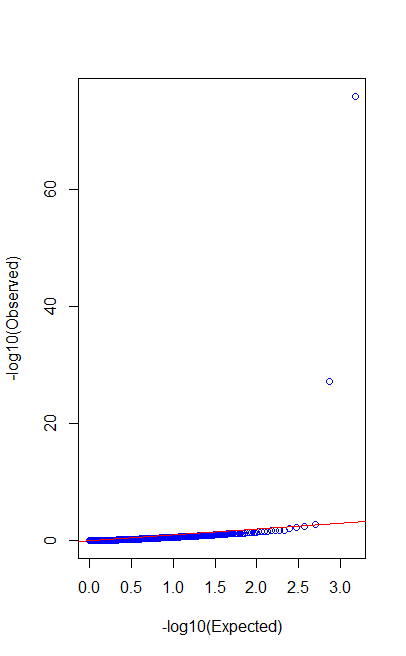
\includegraphics{qqplot.png}
\caption{Quantile-Quantile plot.}\end{figure}

TASSEL detected two of the three QTL: 2 and 20.
The Q-values are 4.1451249e-25 and 1.606586e-73 respectively.

Two observations that are immediately obvious:
\begin{enumerate}
\item {} 
there is almost no difference between allele effects at locus 10

\item {} 
locus 10 is very close to 2 and 20 which might mute its already small effect

\end{enumerate}


\chapter{Indices and tables}
\label{contents:indices-and-tables}\begin{itemize}
\item {} 
\DUspan{xref,std,std-ref}{genindex}

\item {} 
\DUspan{xref,std,std-ref}{modindex}

\item {} 
\DUspan{xref,std,std-ref}{search}

\end{itemize}



\renewcommand{\indexname}{Index}
\printindex
\end{document}
